\section{Konvexe Hülle}
\subsection{Einleitung}
\begin{frame}
	\frametitle{{Konvexe Hülle}}
	\begin{block} {Definition}
	Die \textbf{konvexe Hülle} in einem d-dimensionalen Raum mit n-Punkten ist die kleinste konvexe Menge, die alle n Punkte enthält
	\end{block}
	\pause
	\textbf{Konvexe Mengen} sind geometrische Figuren, die alle Verbindungsstrecken zwischen paarweise verschiedenen Punkten enthalten.
	\visible<3>{
	\begin{figure}
		\mbox{
			\subfigure[\tiny{konvex}]{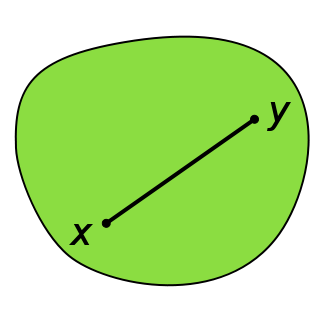
\includegraphics[width=.2\linewidth]{bilder/konvexeMenge.png}}\quad
			\hspace{1cm}
			\subfigure[\tiny{nicht konvex}]{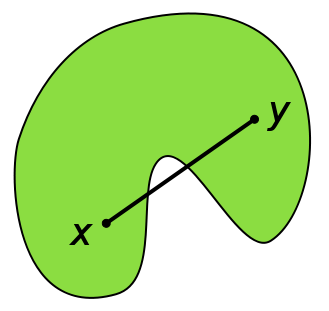
\includegraphics[width=.2\linewidth]{bilder/konvexeMenge2.png}}\quad
			\hspace{1cm}
			\subfigure[\tiny{{vollständiger Graph}}]{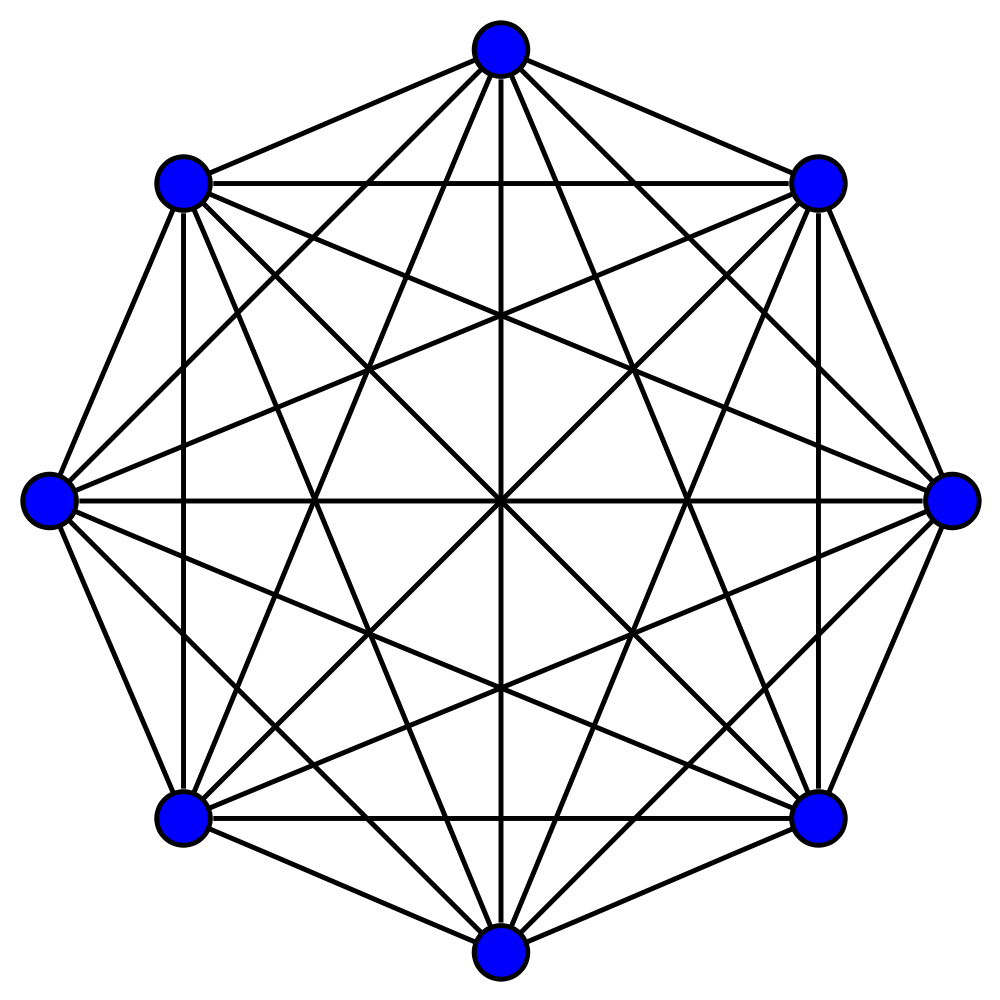
\includegraphics[width=.2\linewidth]{bilder/konvexeMenge3.png}}		
		}
	\end{figure}
	}
\end{frame}

\begin{frame}
	\frametitle{Konvexe Hülle}
\begin{figure}[htbp]
  \centering
  \begin{minipage}[b]{.48\linewidth}
    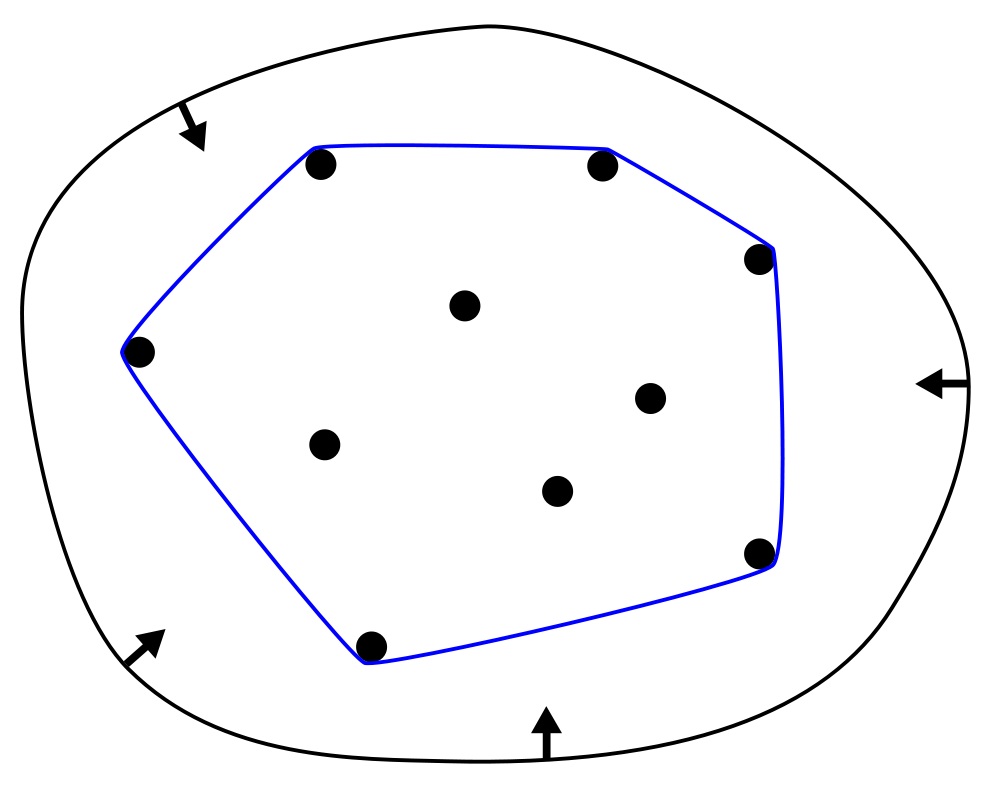
\includegraphics[width=\linewidth]{bilder/konvexeHuelle.png}
  \end{minipage}
  \hfill
  \begin{minipage}[b]{.48\linewidth}
\textbf{Motivation}
\begin{itemize}
	\item Kollisionsberechnung
	\item Voronoi Diagramm
	\item konvexe Optimierung
\end{itemize}
\hspace{0pt}\\\\
\end{minipage}
\end{figure}
\end{frame}



\subsection{Gift Wrapping}
\begin{frame}
	\frametitle{{Gift Wrapping}}
\begin{figure}[htbp]
	\begin{center}
  	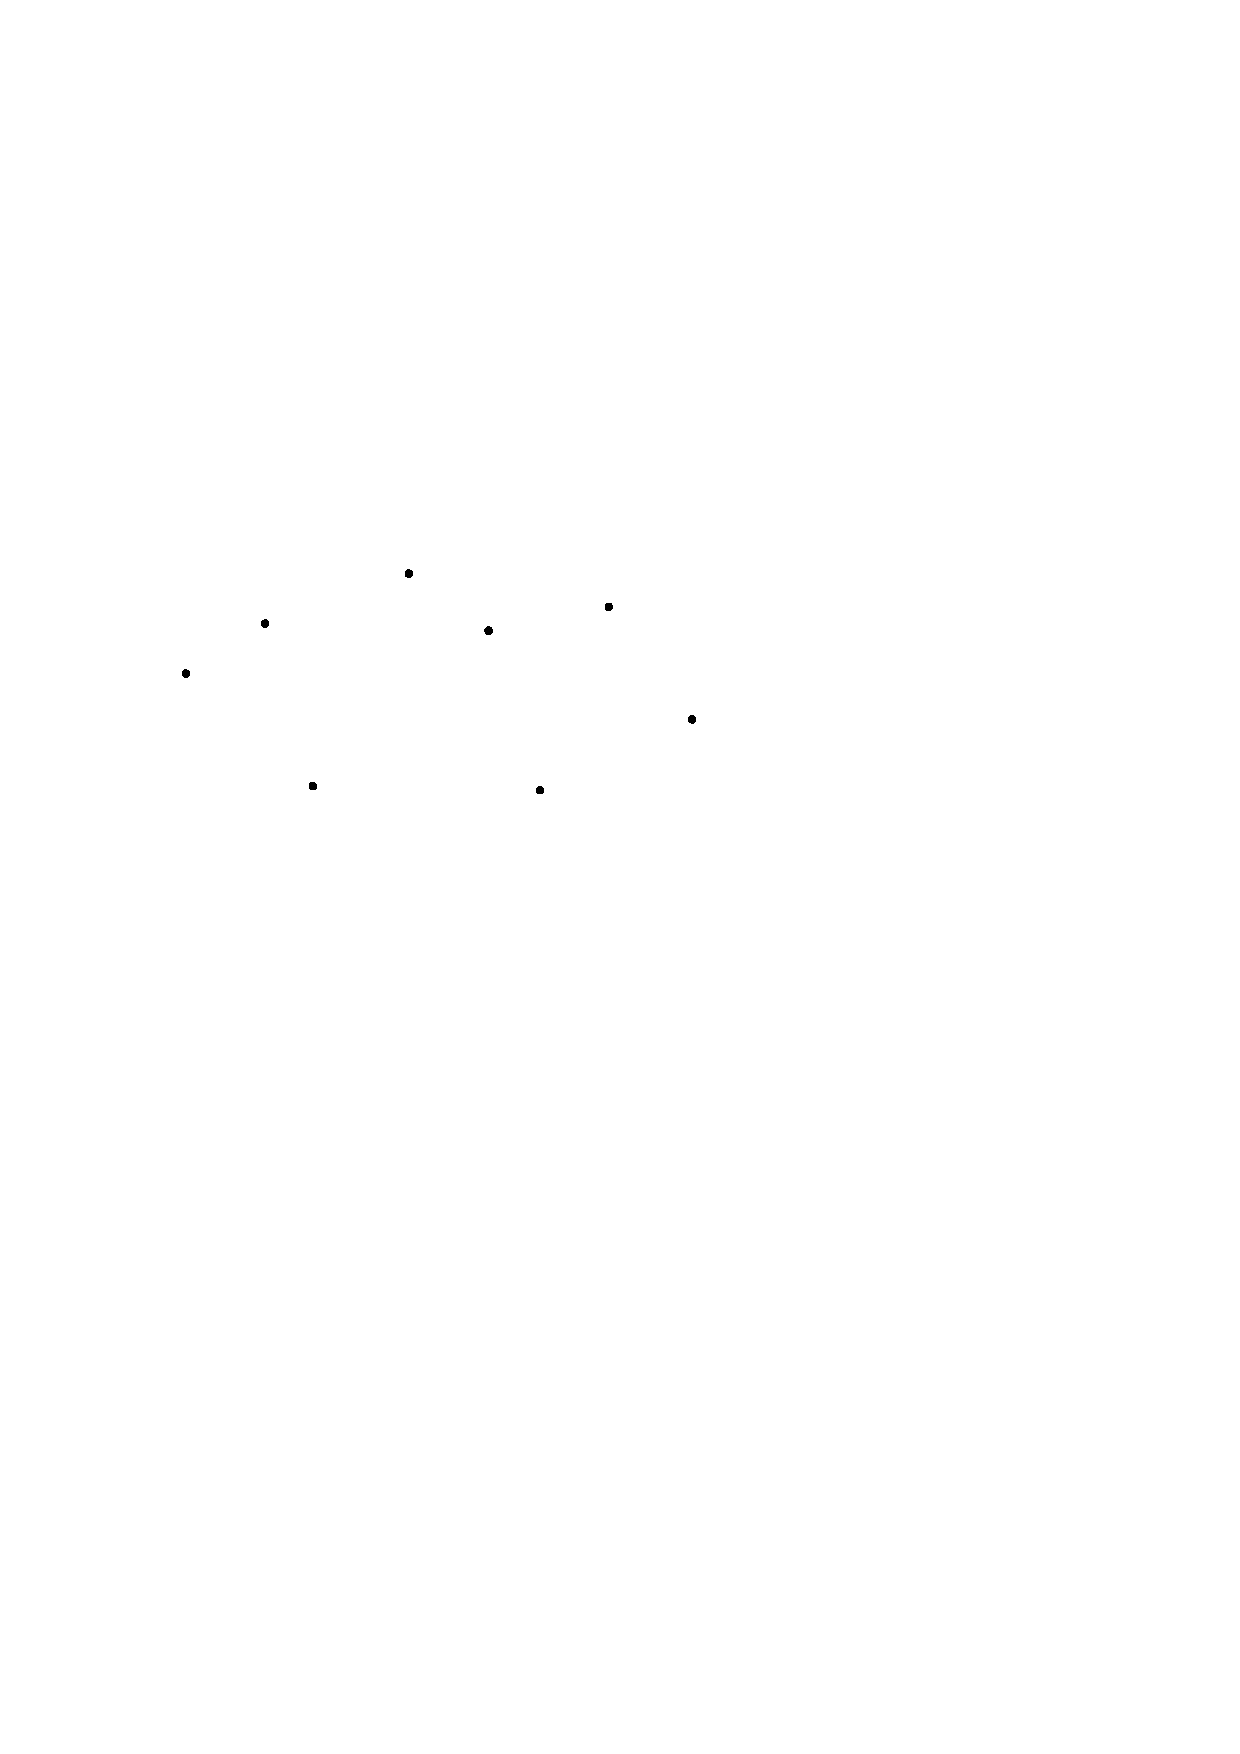
\includegraphics[width=.8\linewidth]{bilder/punkte}
	\end{center}
\end{figure}
\end{frame}

\begin{frame}
	\frametitle{{Gift Wrapping}}
\begin{figure}[htbp]
	\begin{center}
  	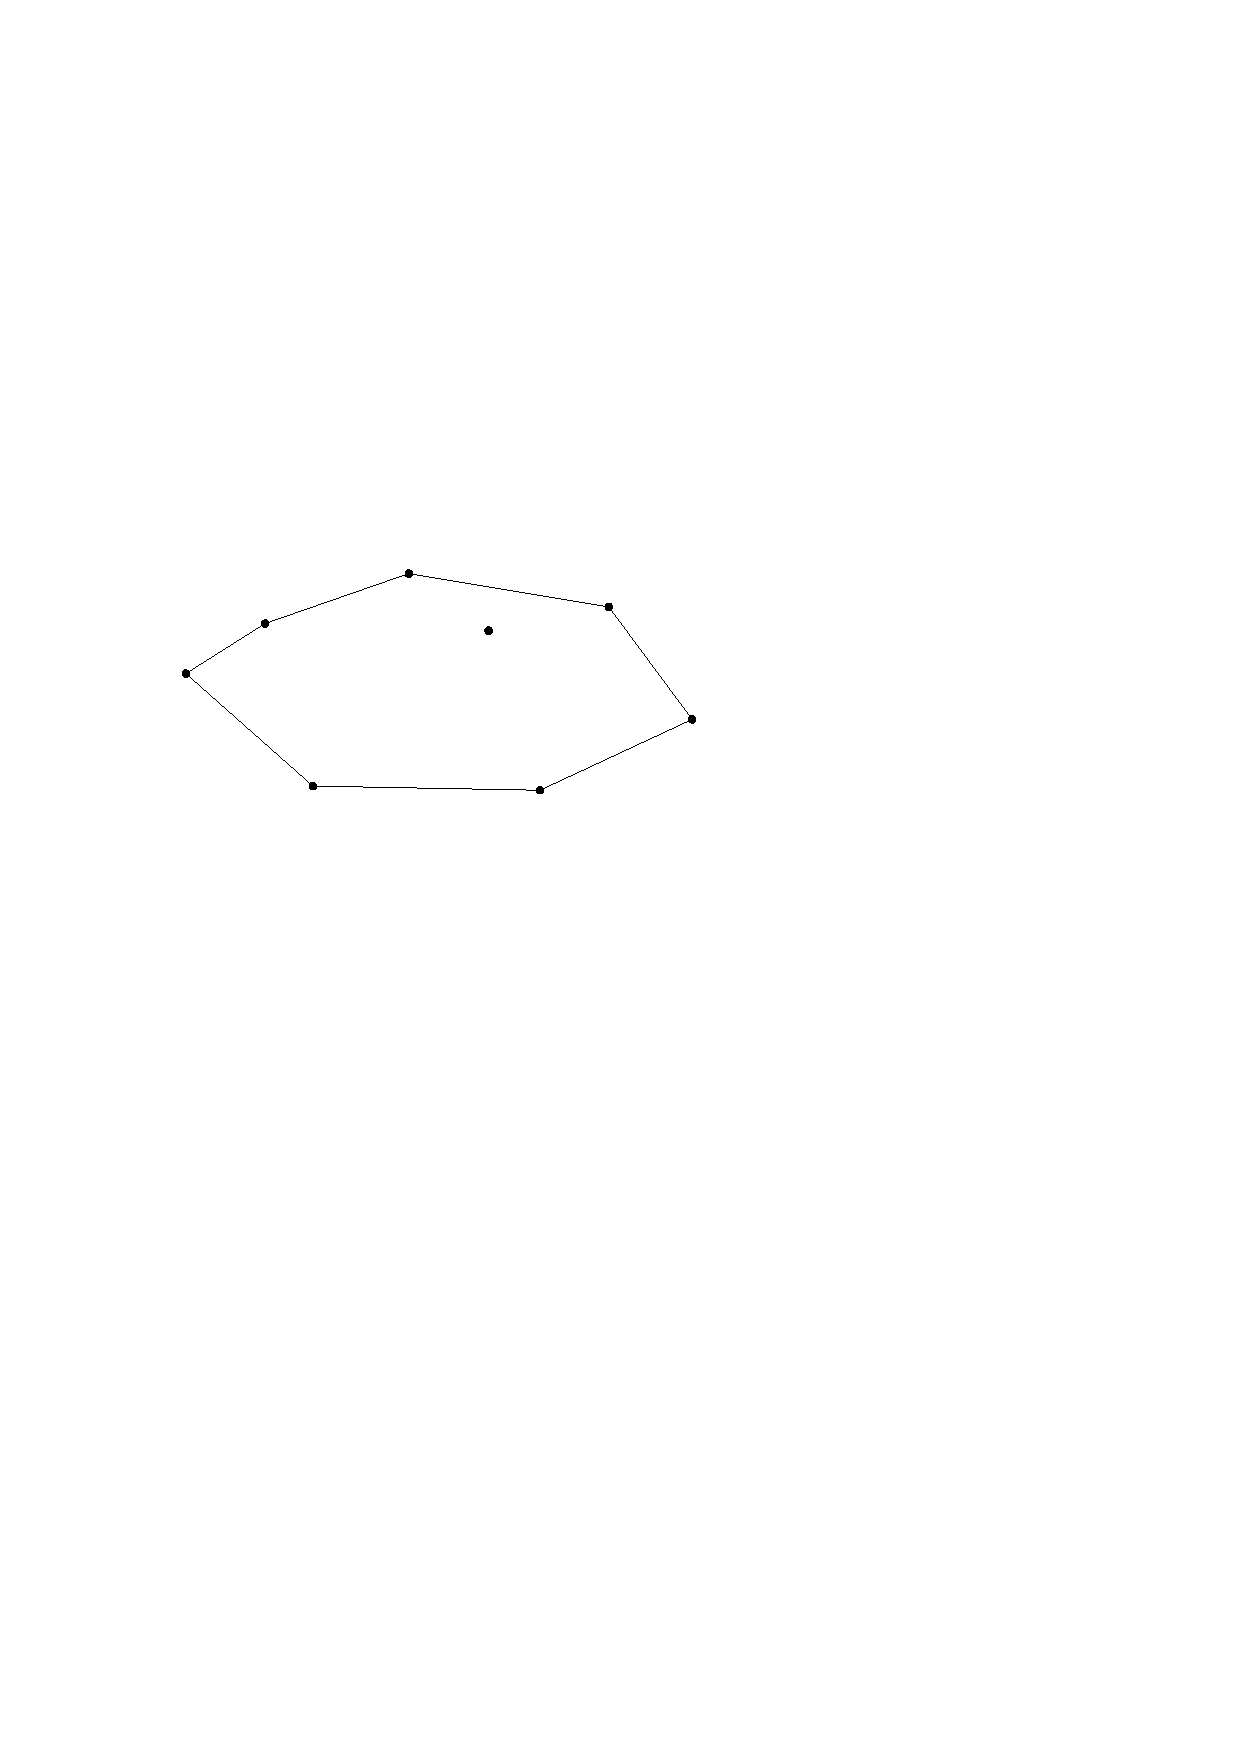
\includegraphics[width=.8\linewidth]{bilder/punkteHulle}
	\end{center}
\end{figure}
\end{frame}


\begin{frame}
	\frametitle{{Gift Wrapping}}
\begin{figure}[htbp]
	\begin{center}
  	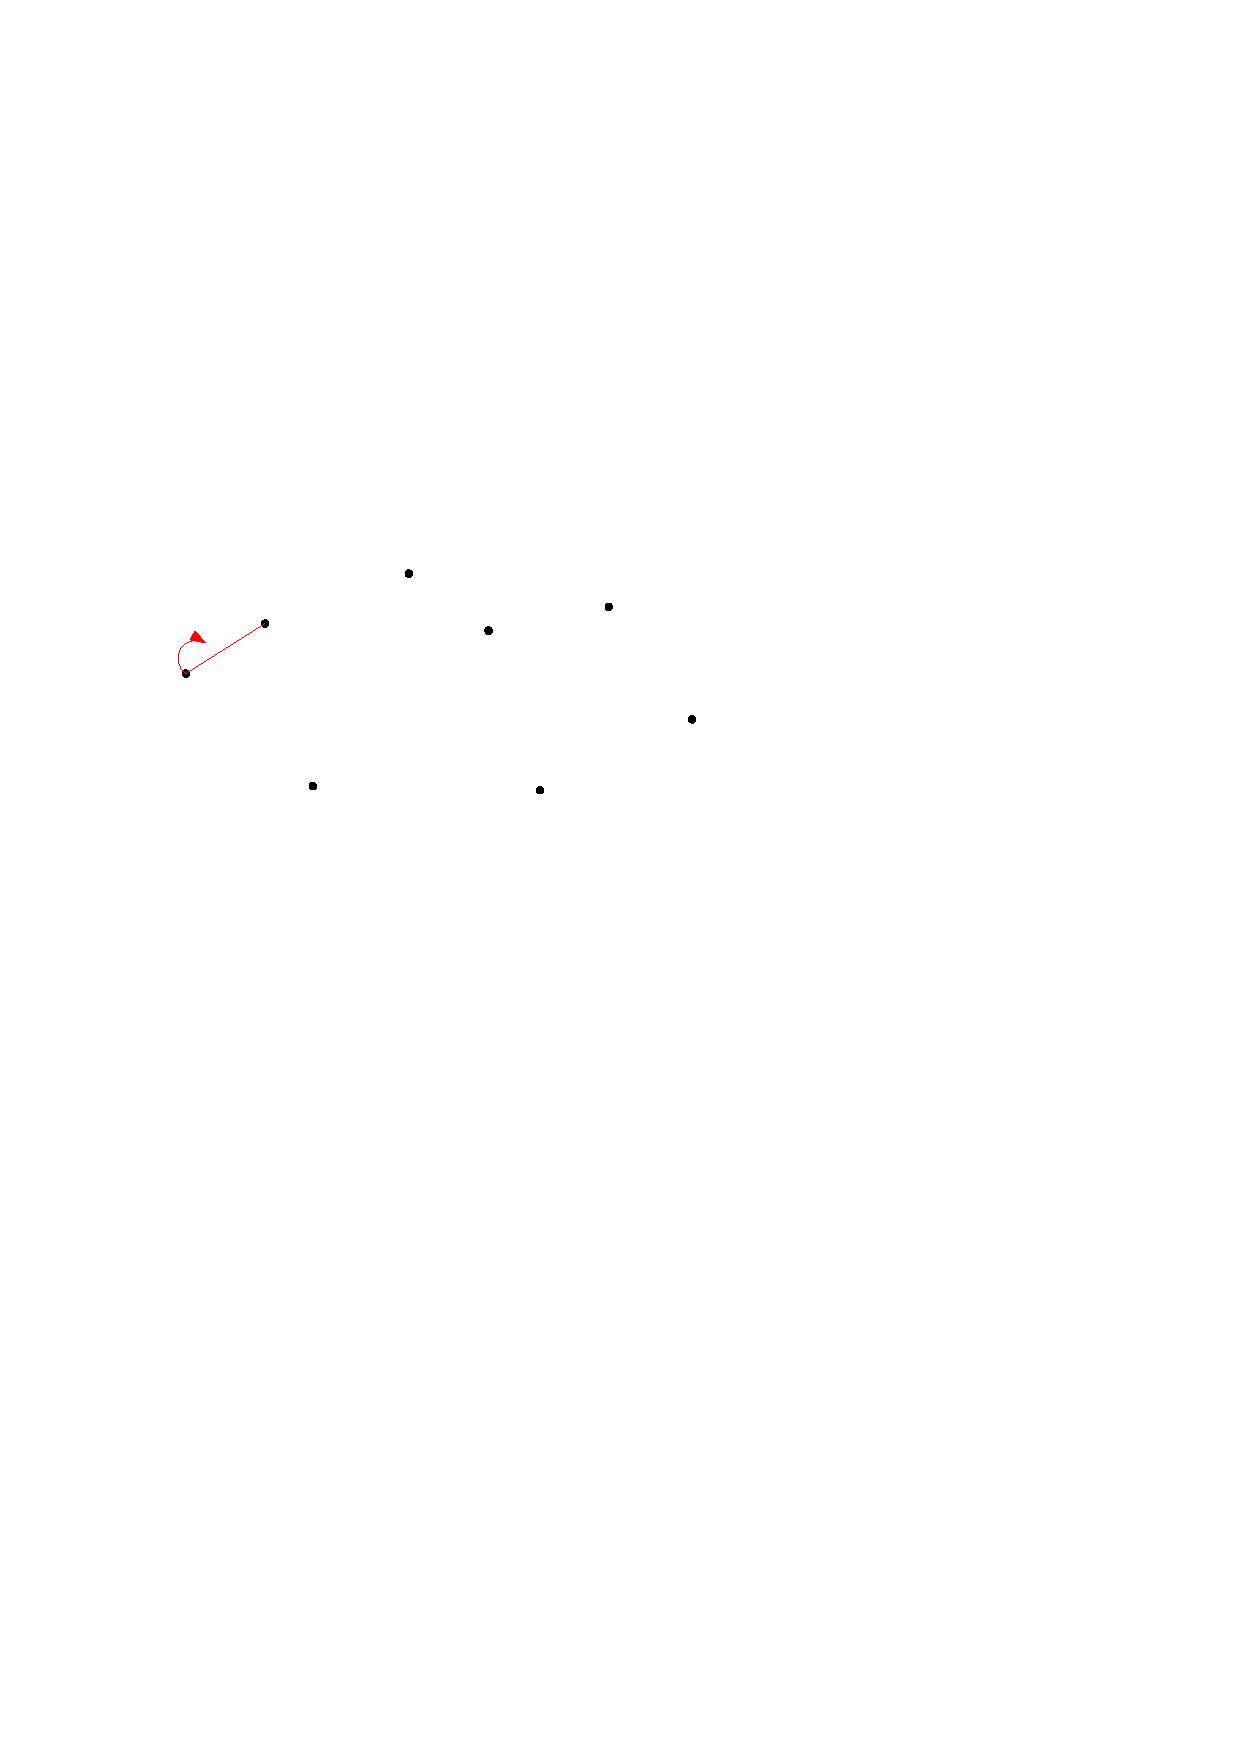
\includegraphics[width=.8\linewidth]{bilder/giftwrap1}
	\end{center}
\end{figure}
\end{frame}


\begin{frame}
	\frametitle{{Gift Wrapping}}
\begin{figure}[htbp]
	\begin{center}
  	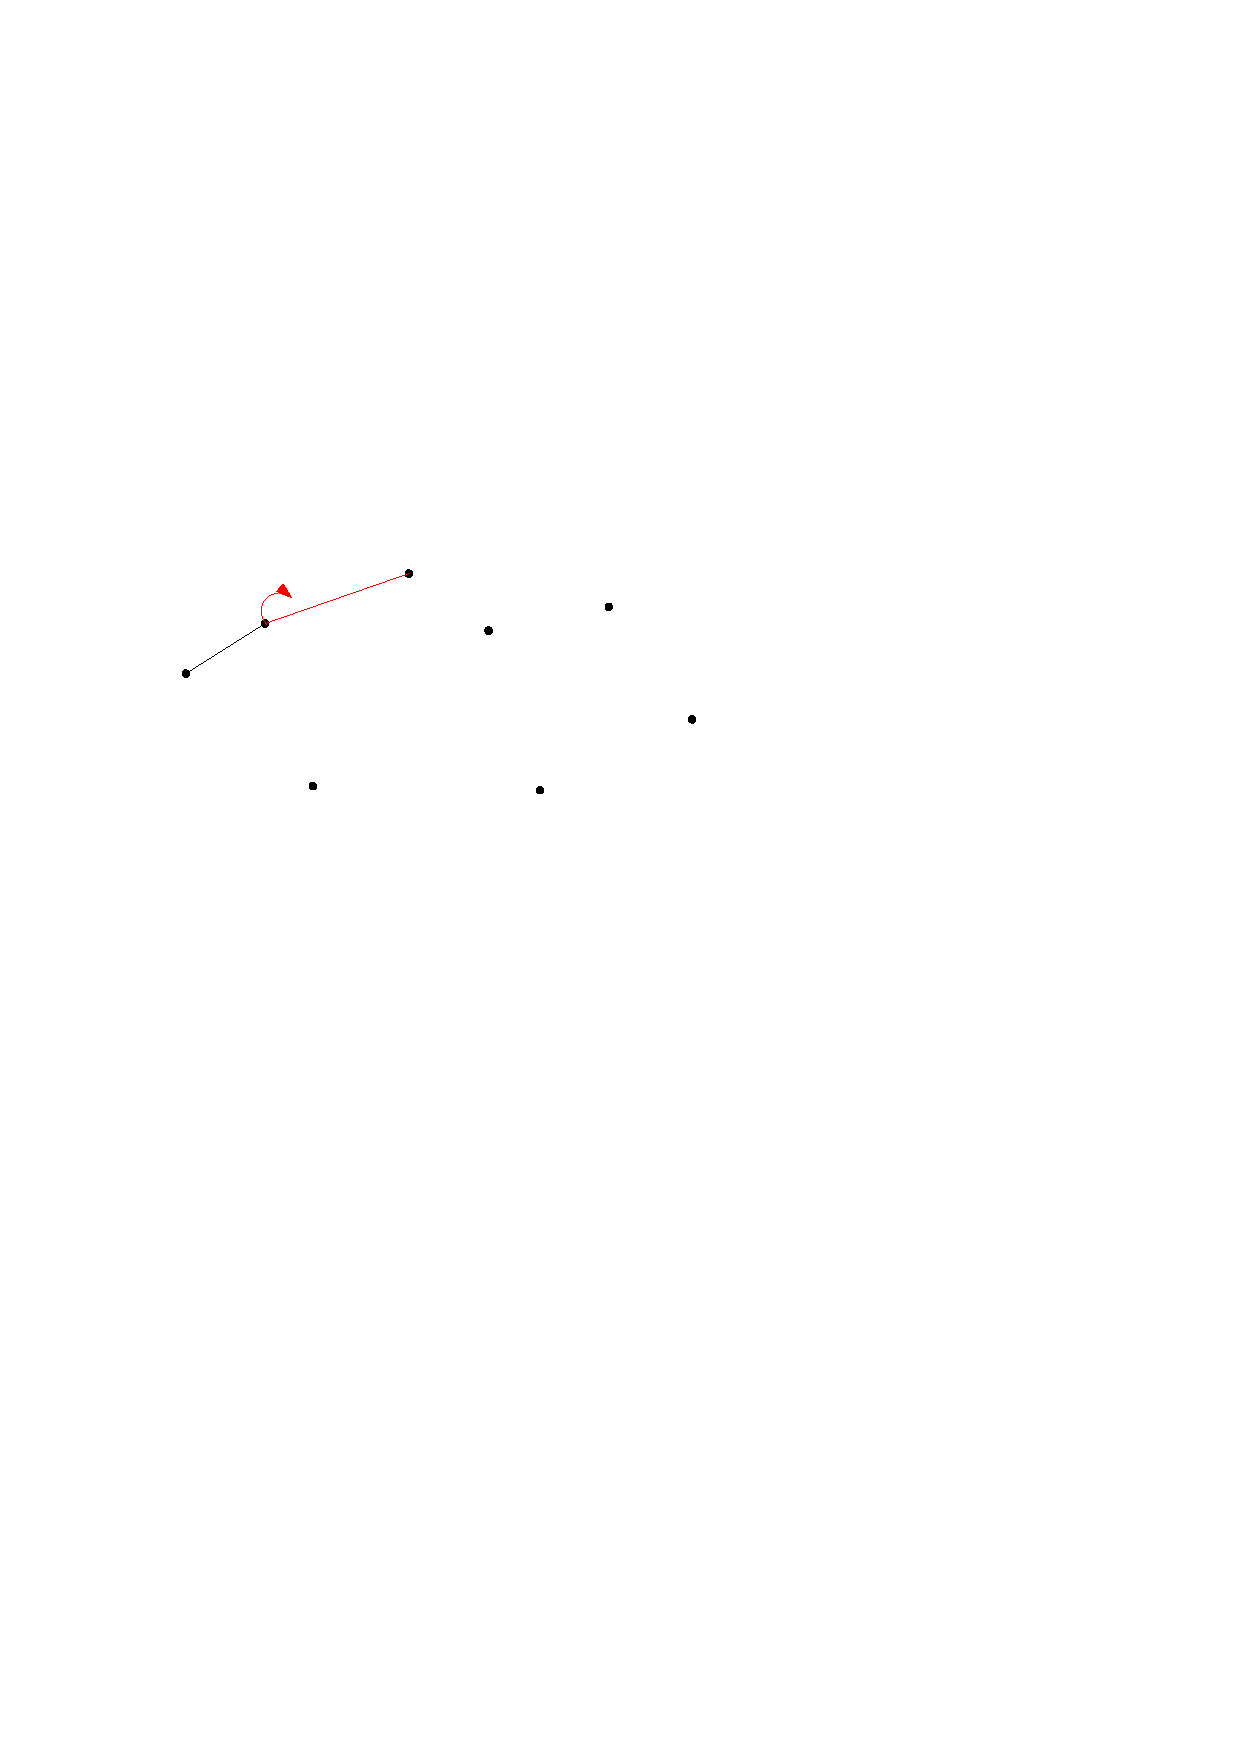
\includegraphics[width=.8\linewidth]{bilder/giftwrap2}
	\end{center}
\end{figure}
\end{frame}


\begin{frame}
	\frametitle{{Gift Wrapping}}
\begin{figure}[htbp]
	\begin{center}
  	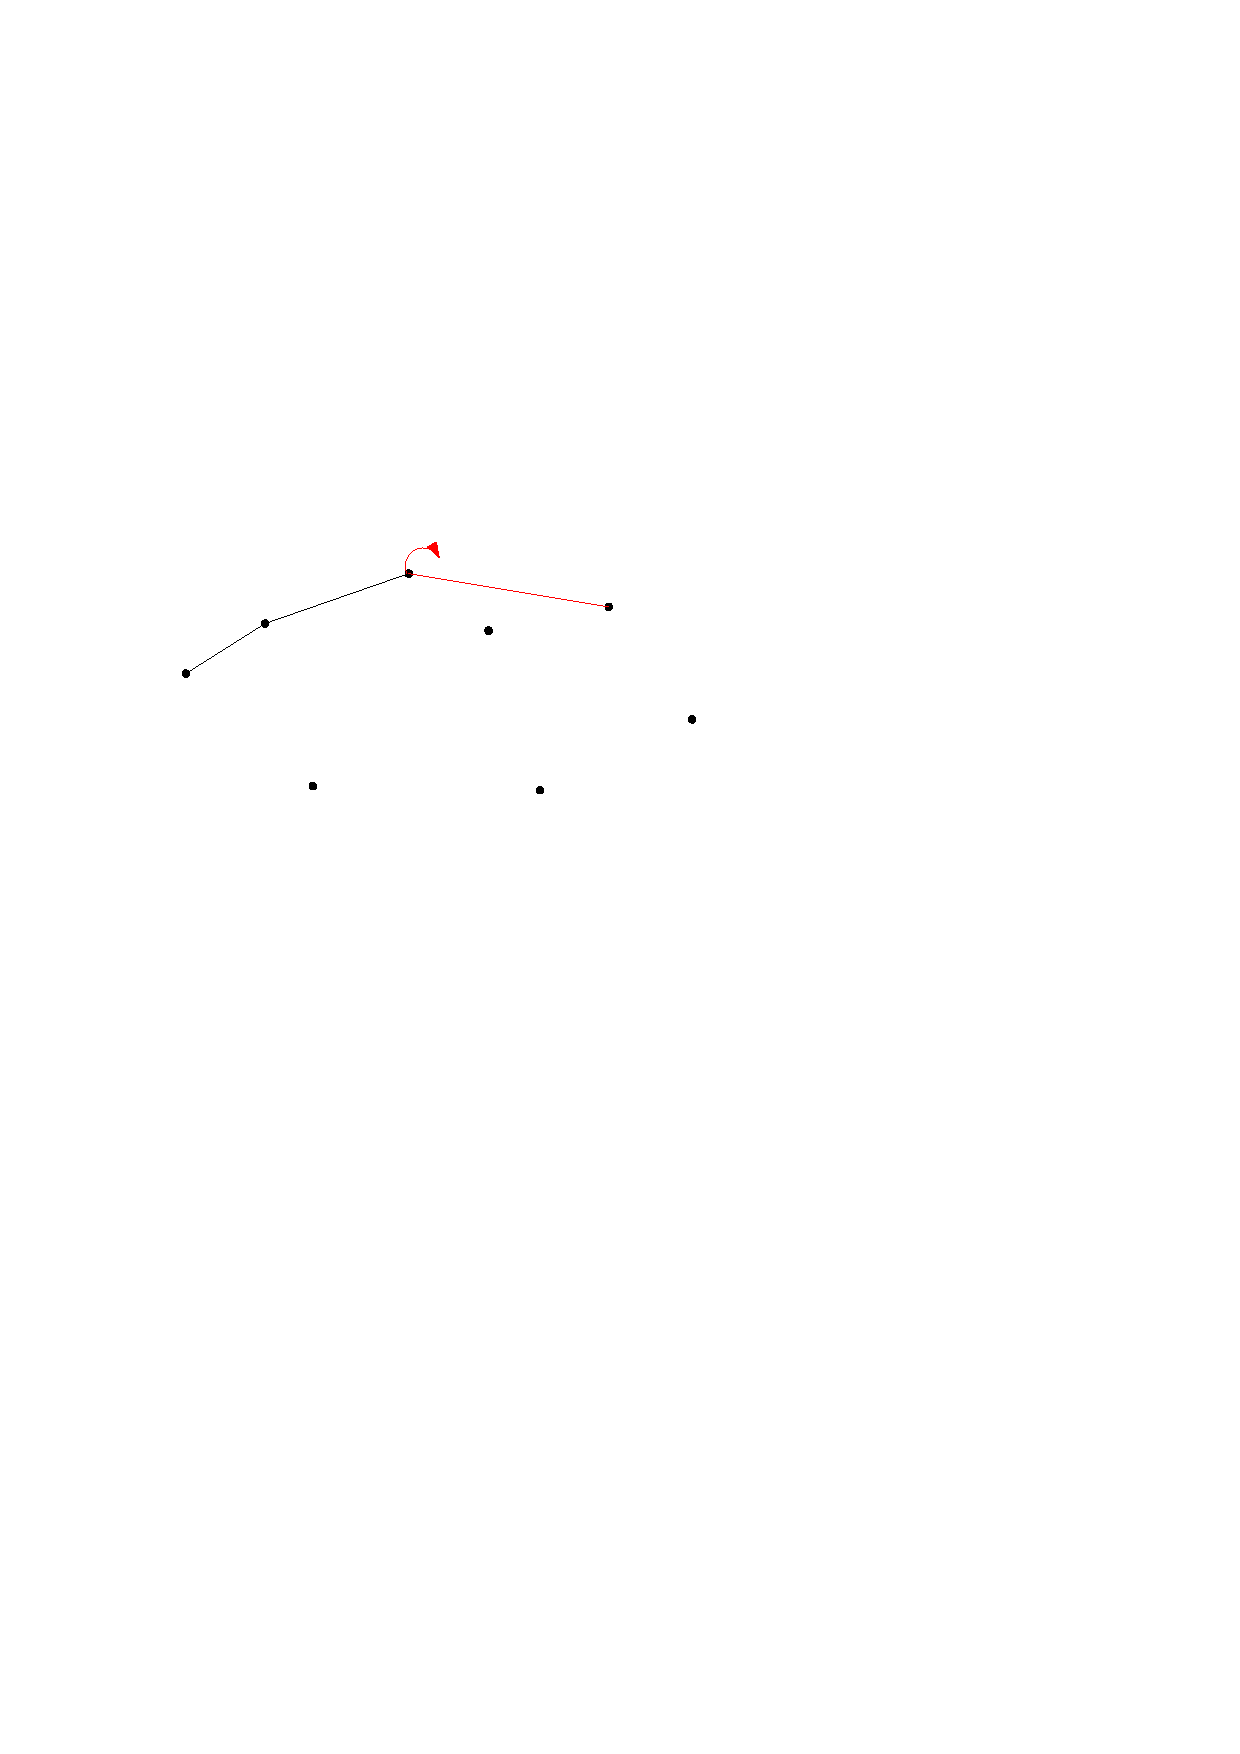
\includegraphics[width=.8\linewidth]{bilder/giftwrap3}
	\end{center}
\end{figure}
\end{frame}


\begin{frame}
	\frametitle{{Gift Wrapping - Pseudocode}}
	\begin{algorithmic}
\State $P\gets \{\mbox{Punkt ganz links}\}$
\State $start\gets \mbox{Punkt ganz links}$
\State $current\gets \mbox{Punkt ganz links}$
\\
\Repeat 
	\For{$p \in P$}
		\If{kein Punkt befindet sich rechts von der Gerade current---p}
			P += p\\
			current = p
		\EndIf
	\EndFor
\Until{current == start}
\end{algorithmic}
$\Rightarrow O(n^2)$
\end{frame}

\subsection{Graham Scan}

\begin{frame}
	\frametitle{Weitere Beobachtungen zu konvexen Hüllen}
\begin{figure}[htbp]
  \centering
  \begin{minipage}[b]{.48\linewidth}
    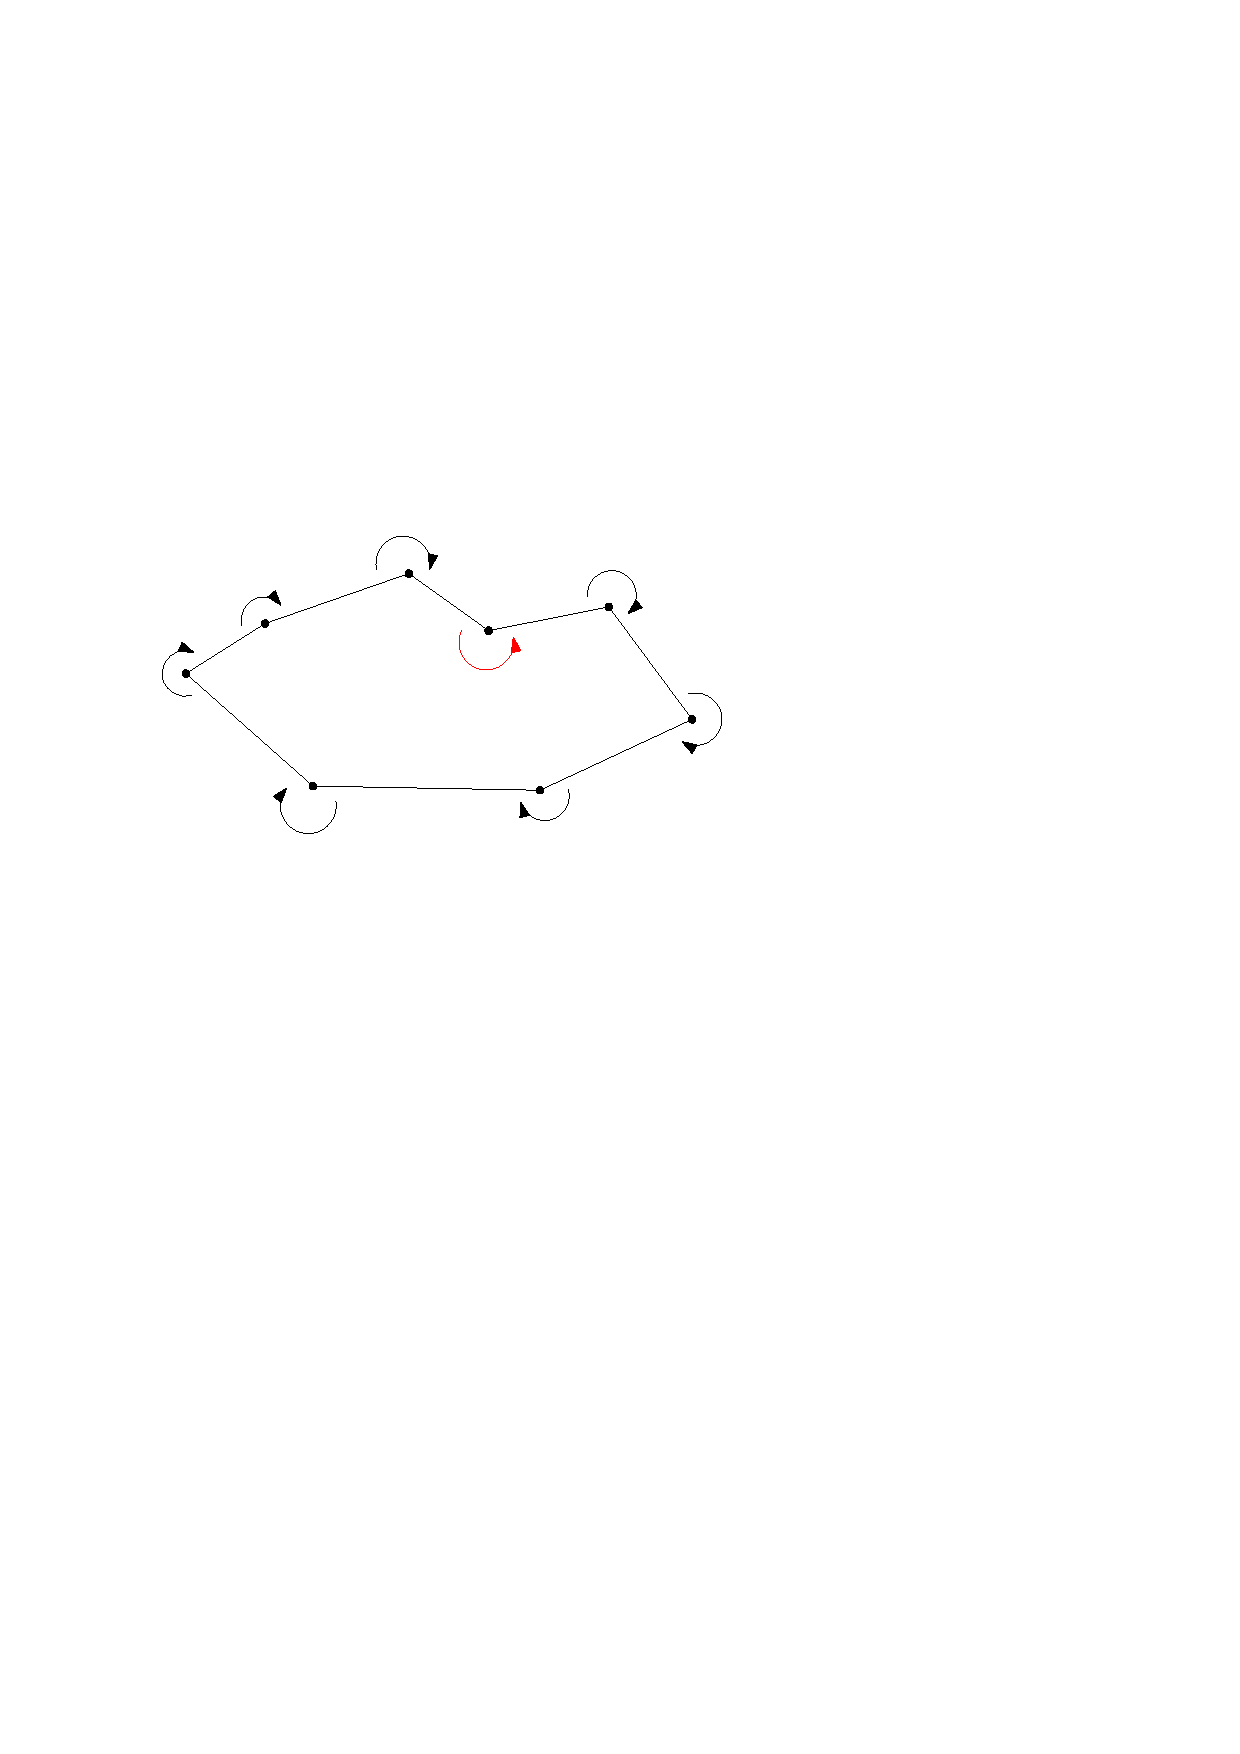
\includegraphics[width=\linewidth]{bilder/nichtKonvexRechts}
    \\
    \\
    \small{Beliebige Hülle mit Rechts- und Linksabbiegungen}
  \end{minipage}
  \hfill
  \pause
  \begin{minipage}[b]{.48\linewidth}
    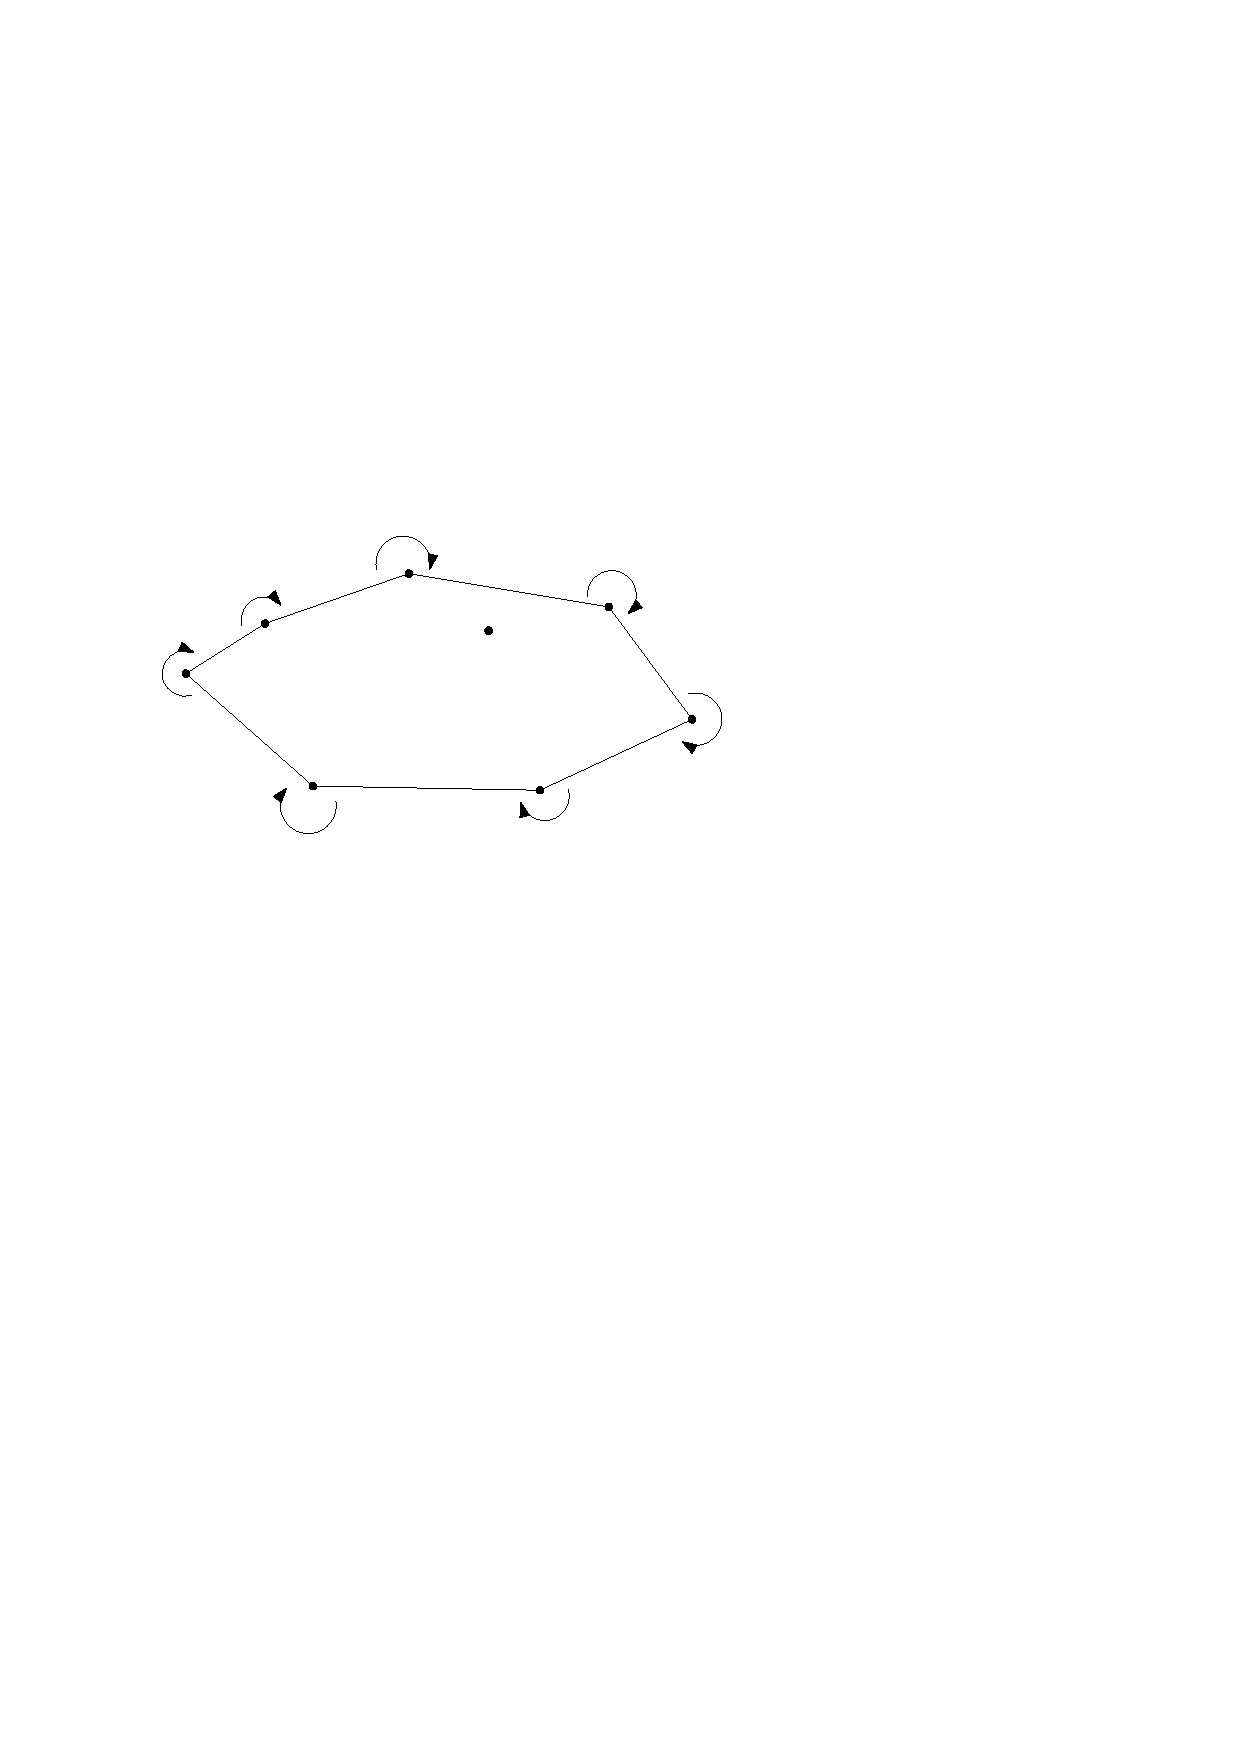
\includegraphics[width=\linewidth]{bilder/konvexRechts}
    \\
    \\
    \small{Konvexe Hülle nur mit Rechtsabbiegungen}
    \end{minipage}
\end{figure}
\pause
$\Rightarrow$ vom Punkt ganz links bis zum Punkt ganz rechts schreitet die konvexe Hülle mit jeder Kante weiter immer weiter nach rechts.
\end{frame}


\begin{frame}
	\frametitle{{Graham Scan}}
\begin{figure}[htbp]
	\begin{center}
  	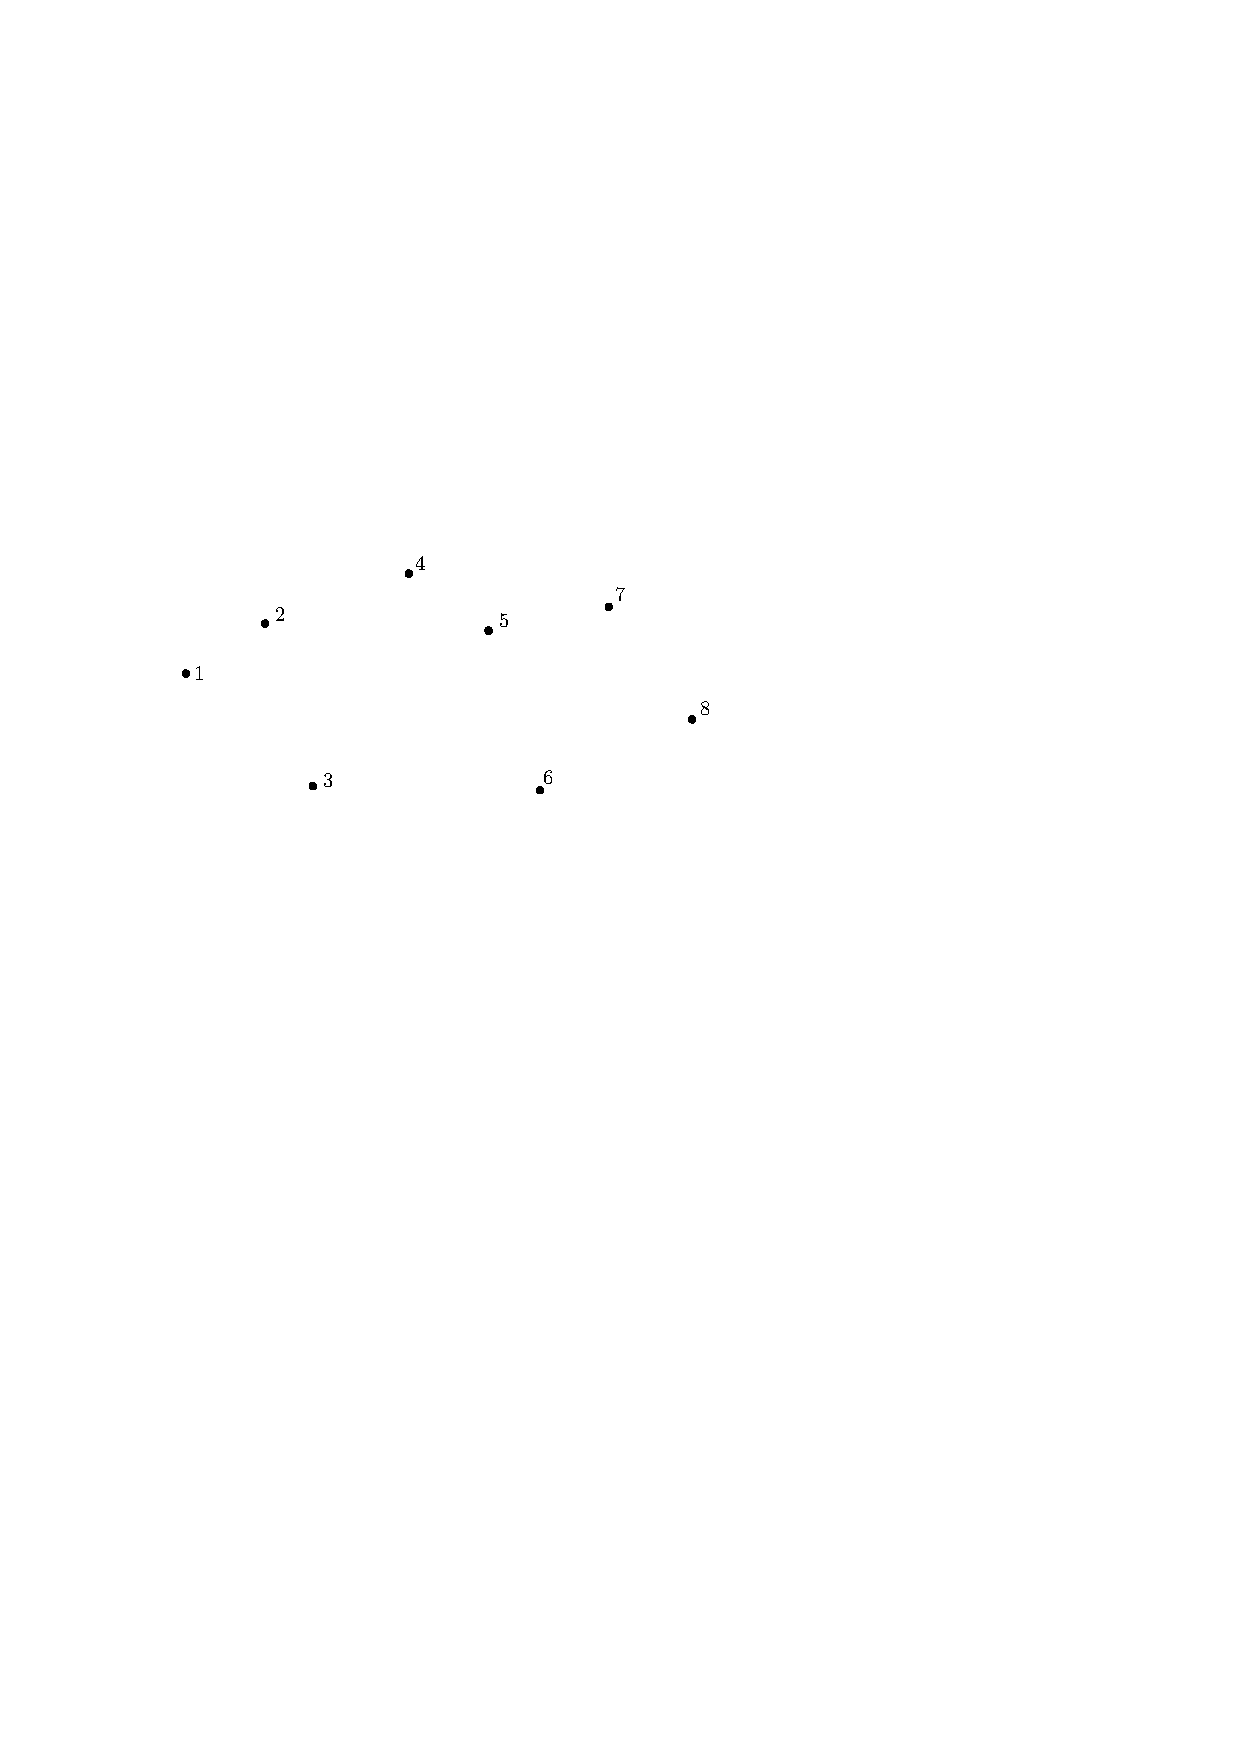
\includegraphics[width=.8\linewidth]{bilder/graham1}
	\end{center}
\end{figure}
\end{frame}


\begin{frame}
	\frametitle{{Graham Scan}}
\begin{figure}[htbp]
	\begin{center}
  	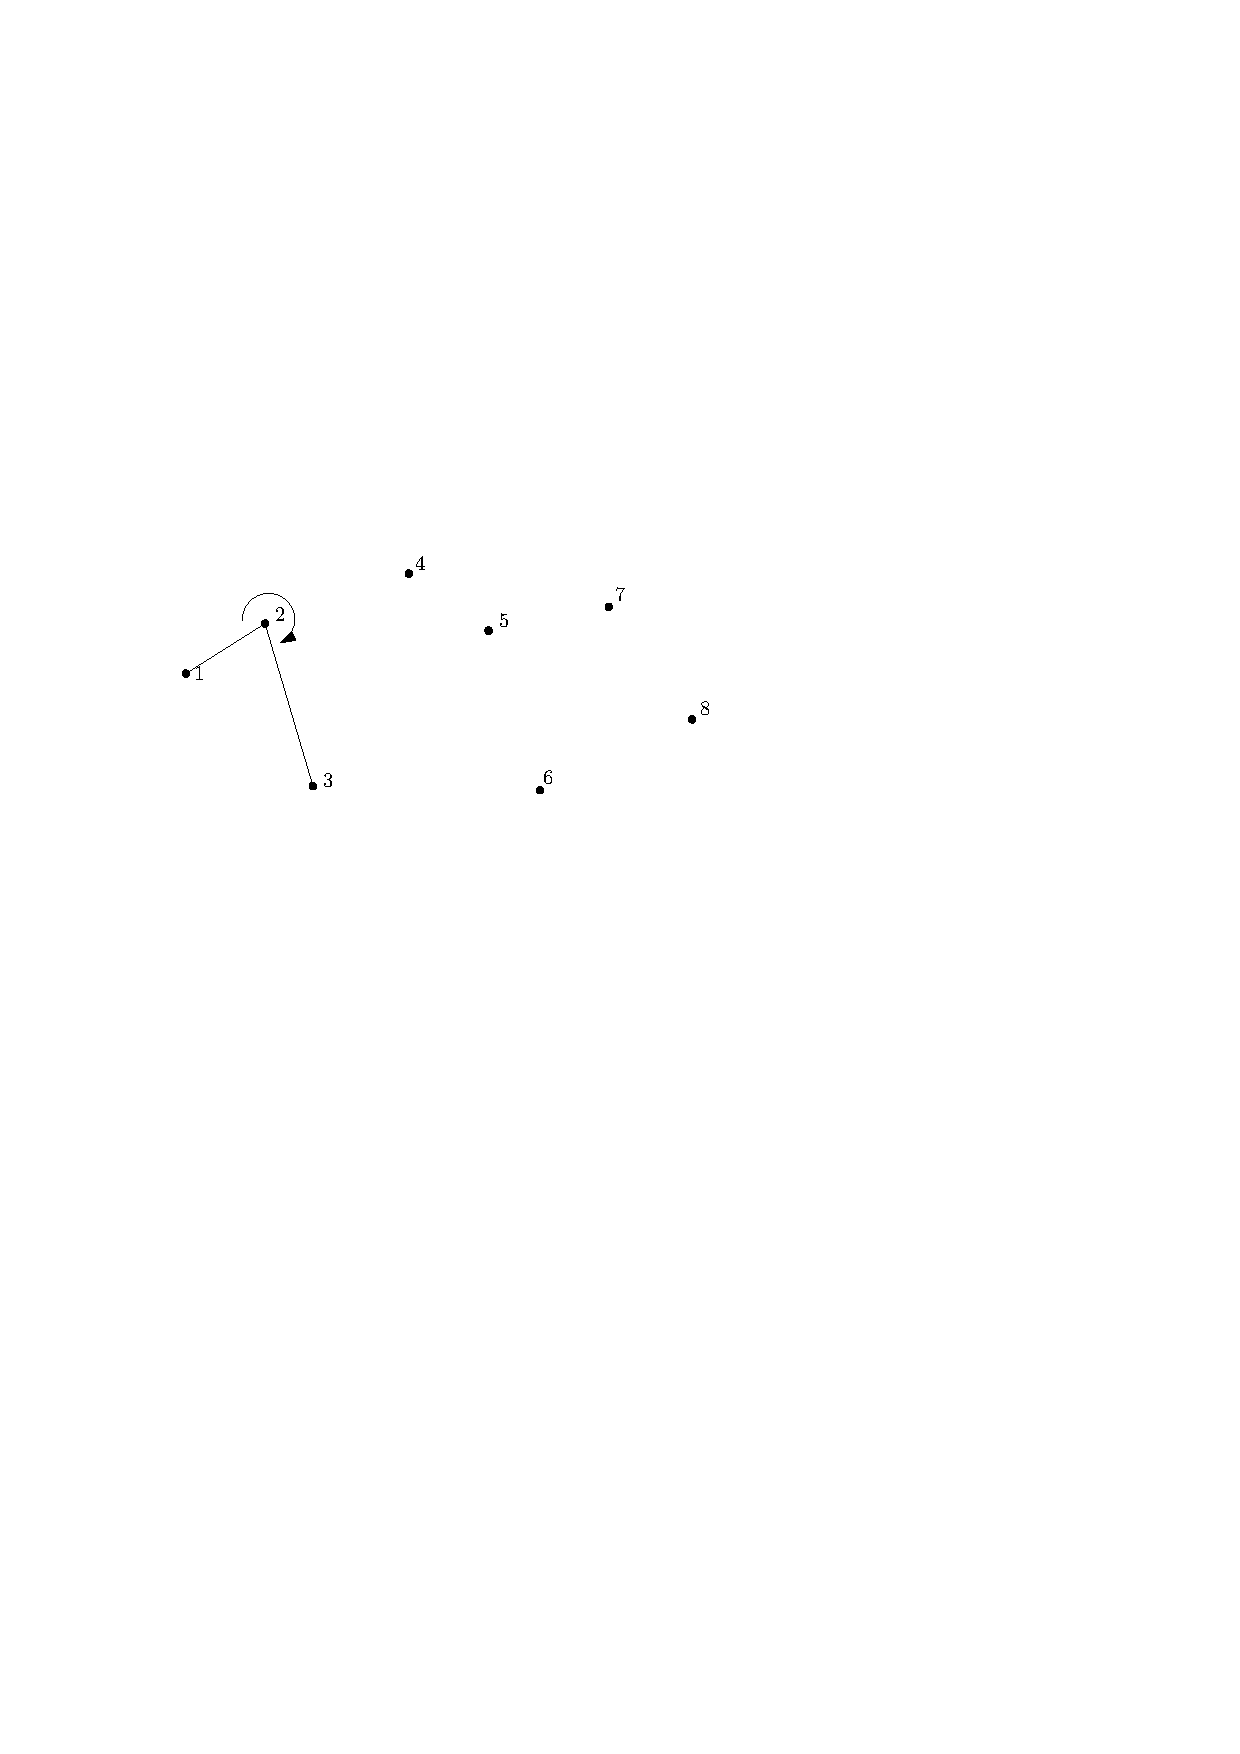
\includegraphics[width=.8\linewidth]{bilder/graham2}
	\end{center}
\end{figure}
\end{frame}


\begin{frame}
	\frametitle{{Graham Scan}}
\begin{figure}[htbp]
	\begin{center}
  	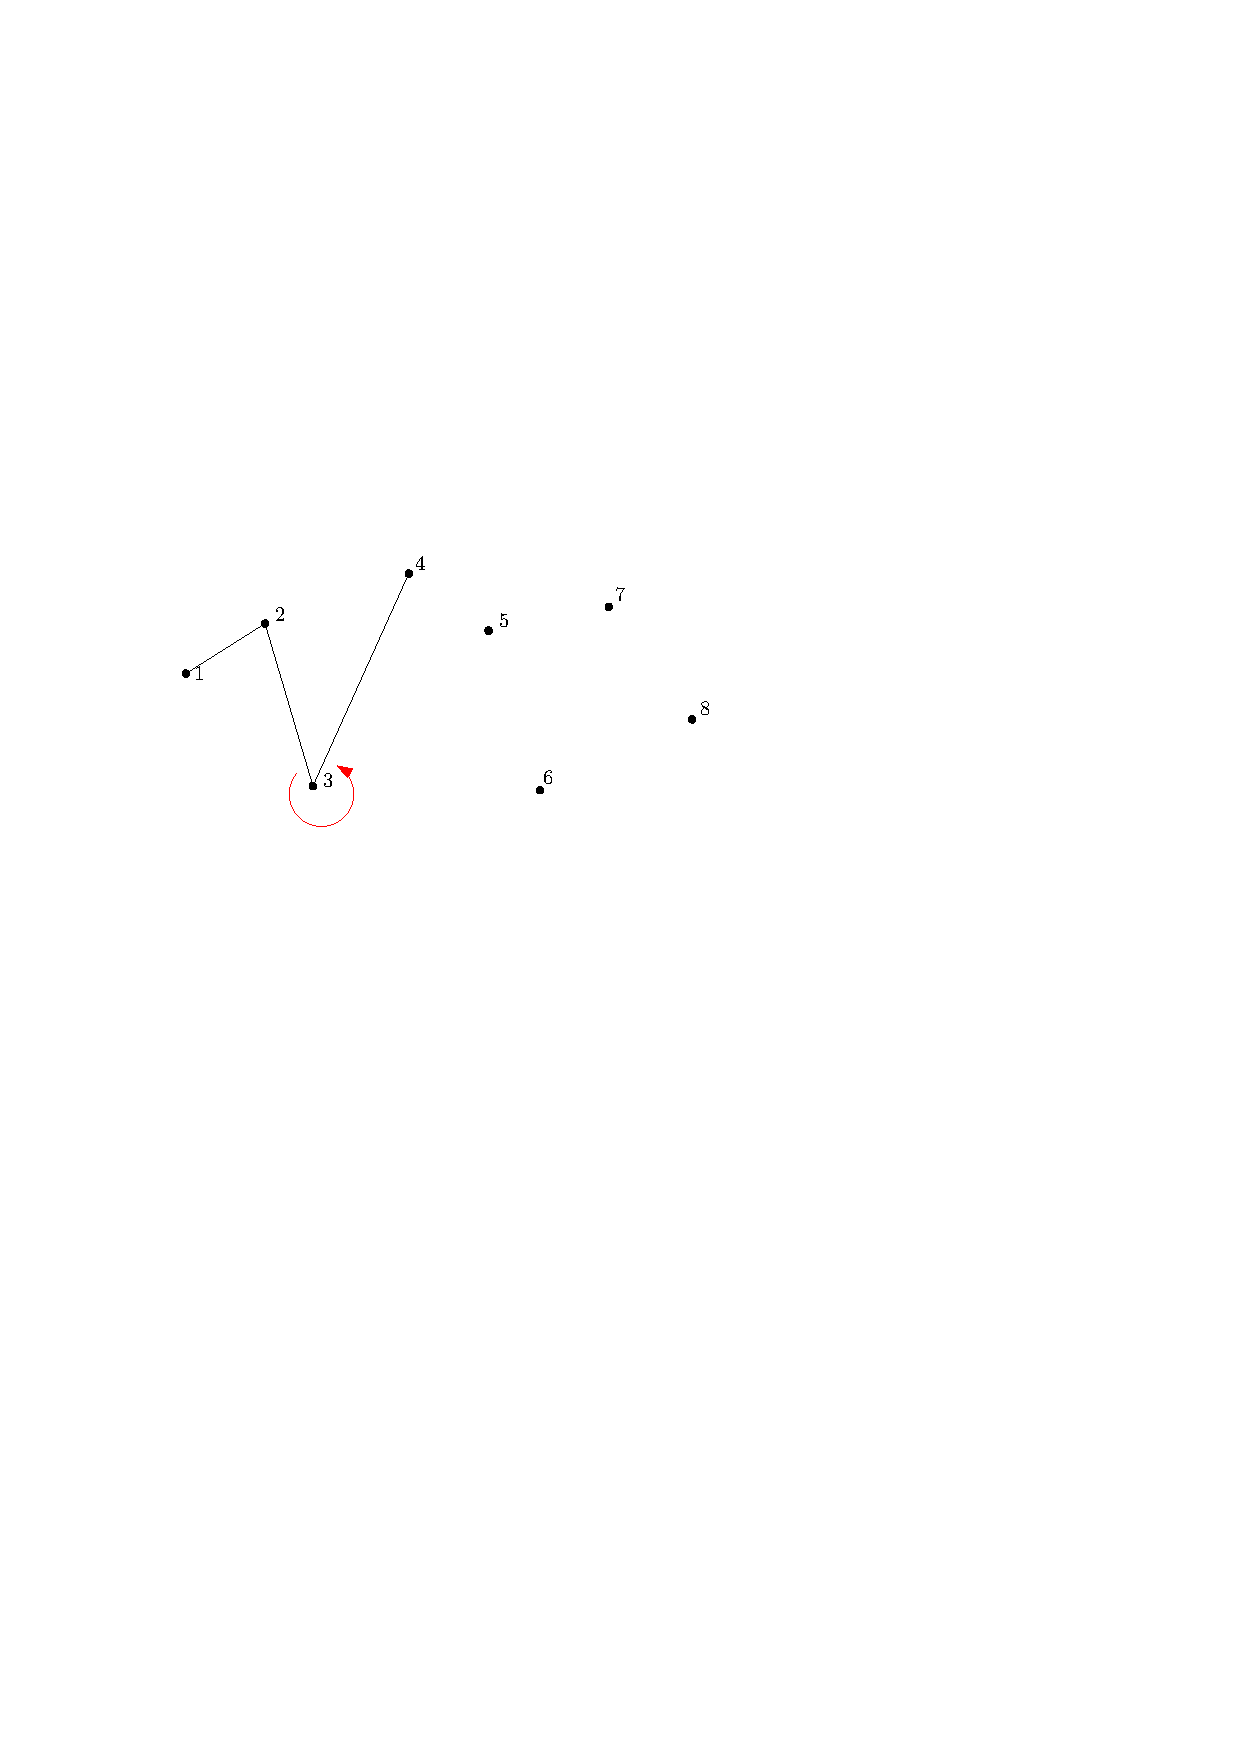
\includegraphics[width=.8\linewidth]{bilder/graham3}
	\end{center}
\end{figure}
\end{frame}


\begin{frame}
	\frametitle{{Graham Scan}}
\begin{figure}[htbp]
	\begin{center}
  	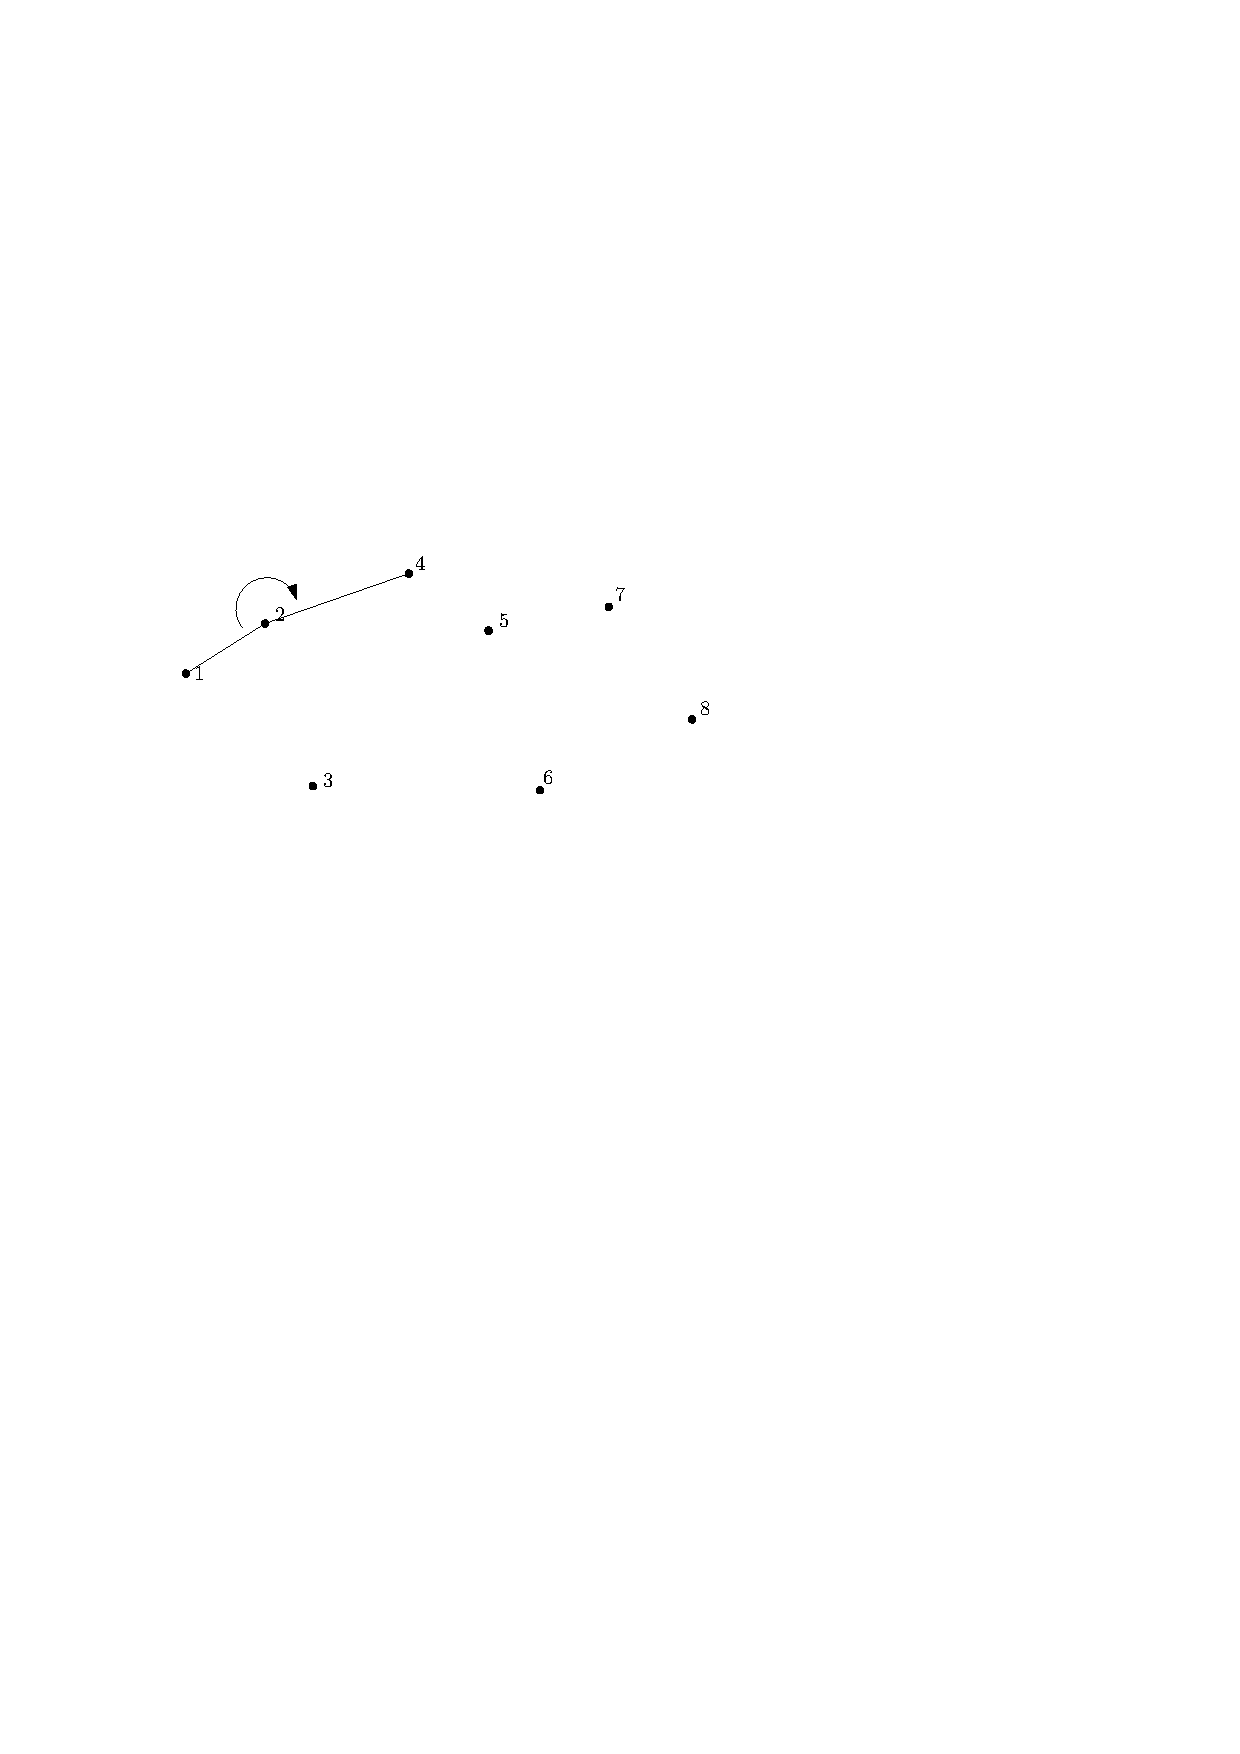
\includegraphics[width=.8\linewidth]{bilder/graham4}
	\end{center}
\end{figure}
\end{frame}


\begin{frame}
	\frametitle{{Graham Scan}}
\begin{figure}[htbp]
	\begin{center}
  	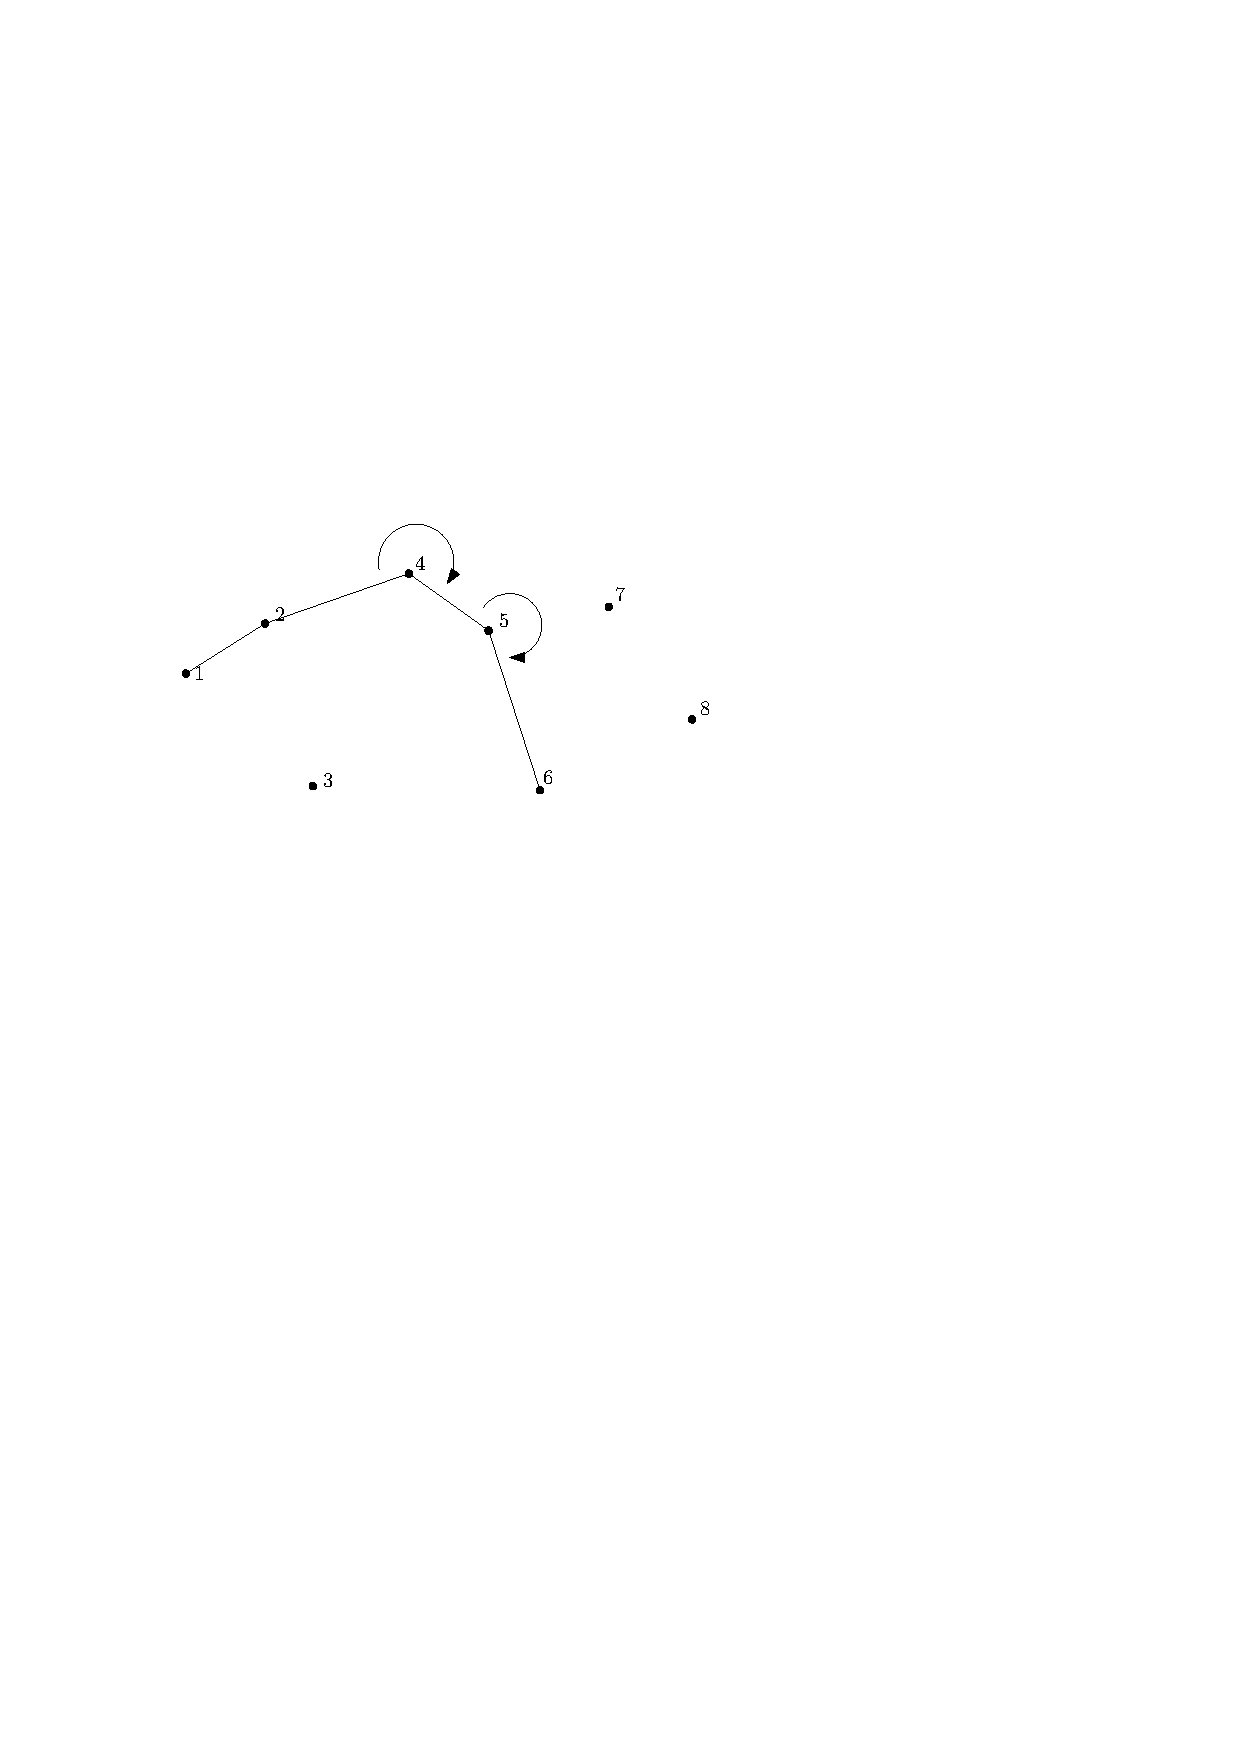
\includegraphics[width=.8\linewidth]{bilder/graham5}
	\end{center}
\end{figure}
\end{frame}


\begin{frame}
	\frametitle{{Graham Scan}}
\begin{figure}[htbp]
	\begin{center}
  	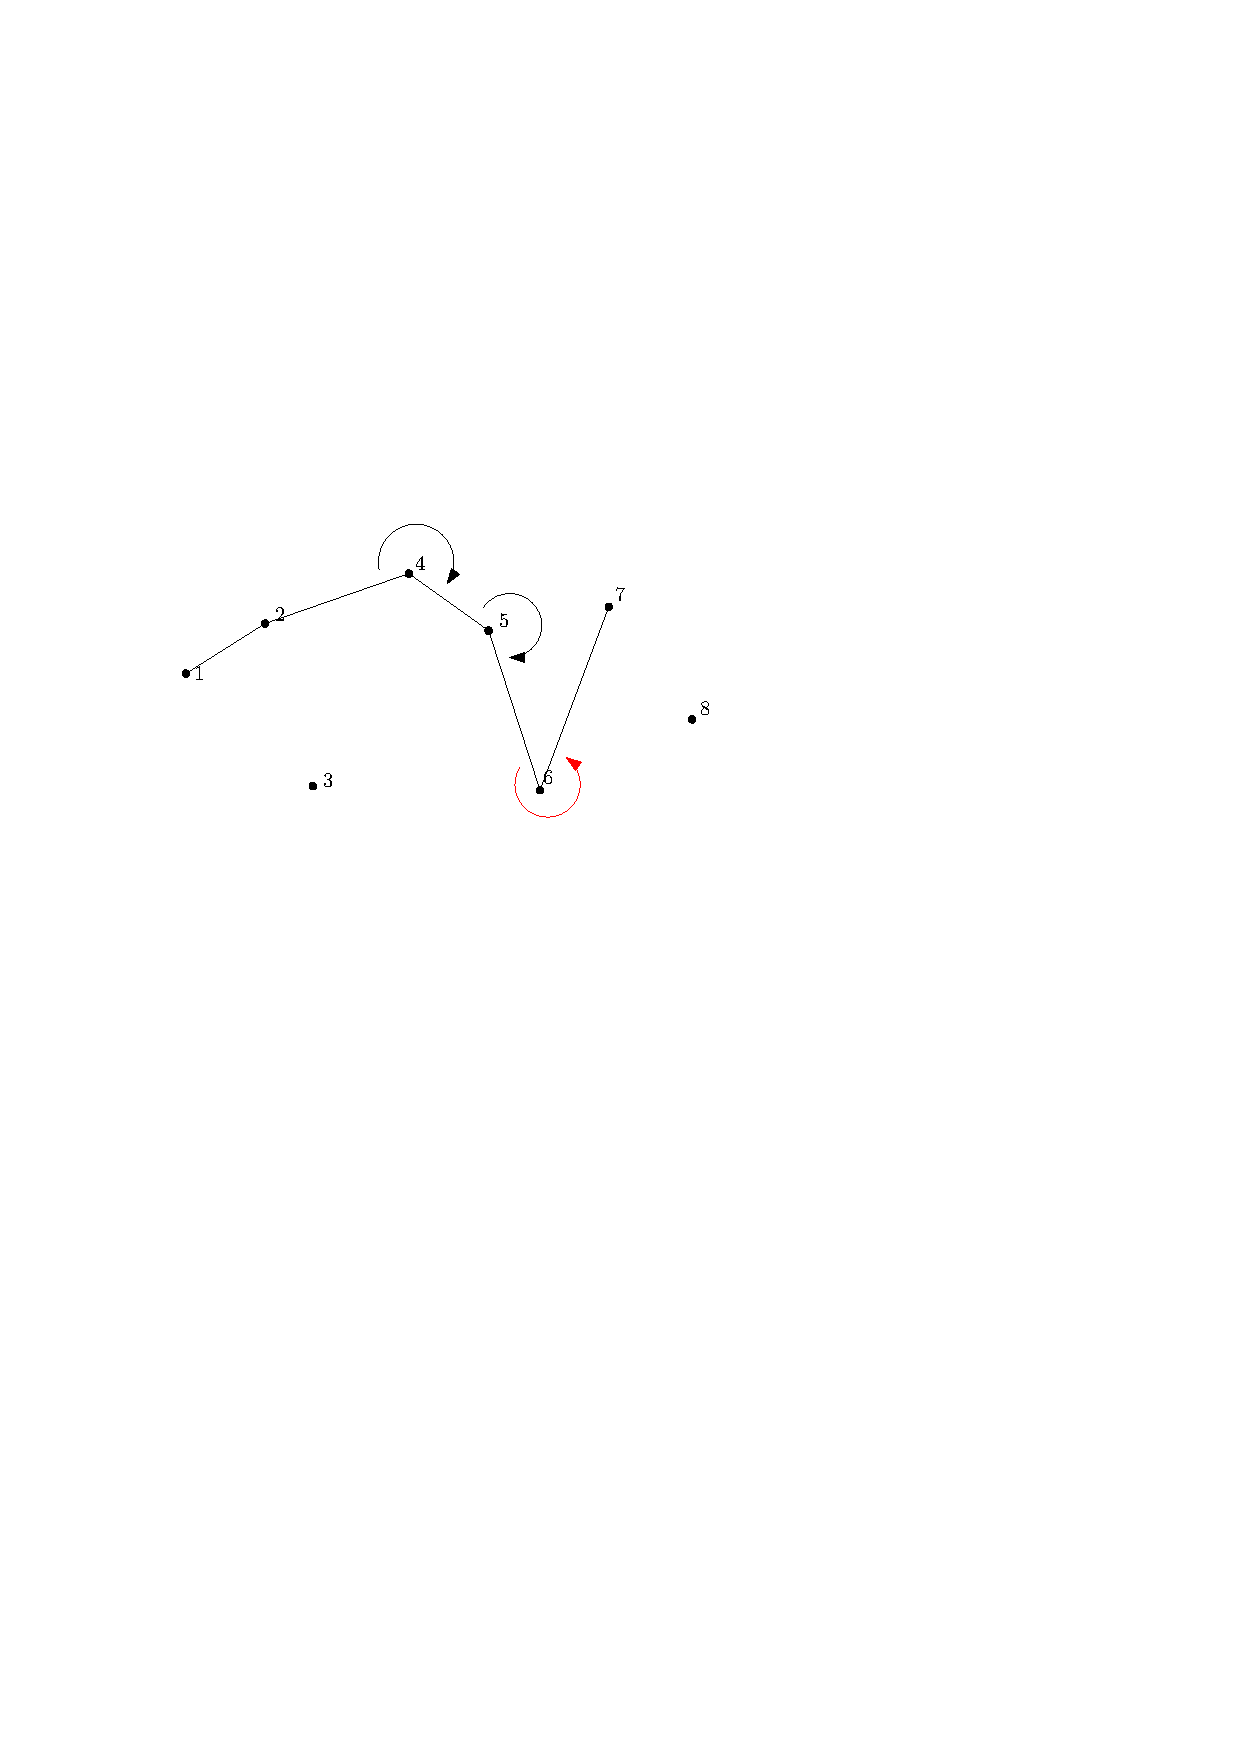
\includegraphics[width=.8\linewidth]{bilder/graham6}
	\end{center}
\end{figure}
\end{frame}


\begin{frame}
	\frametitle{{Graham Scan}}
\begin{figure}[htbp]
	\begin{center}
  	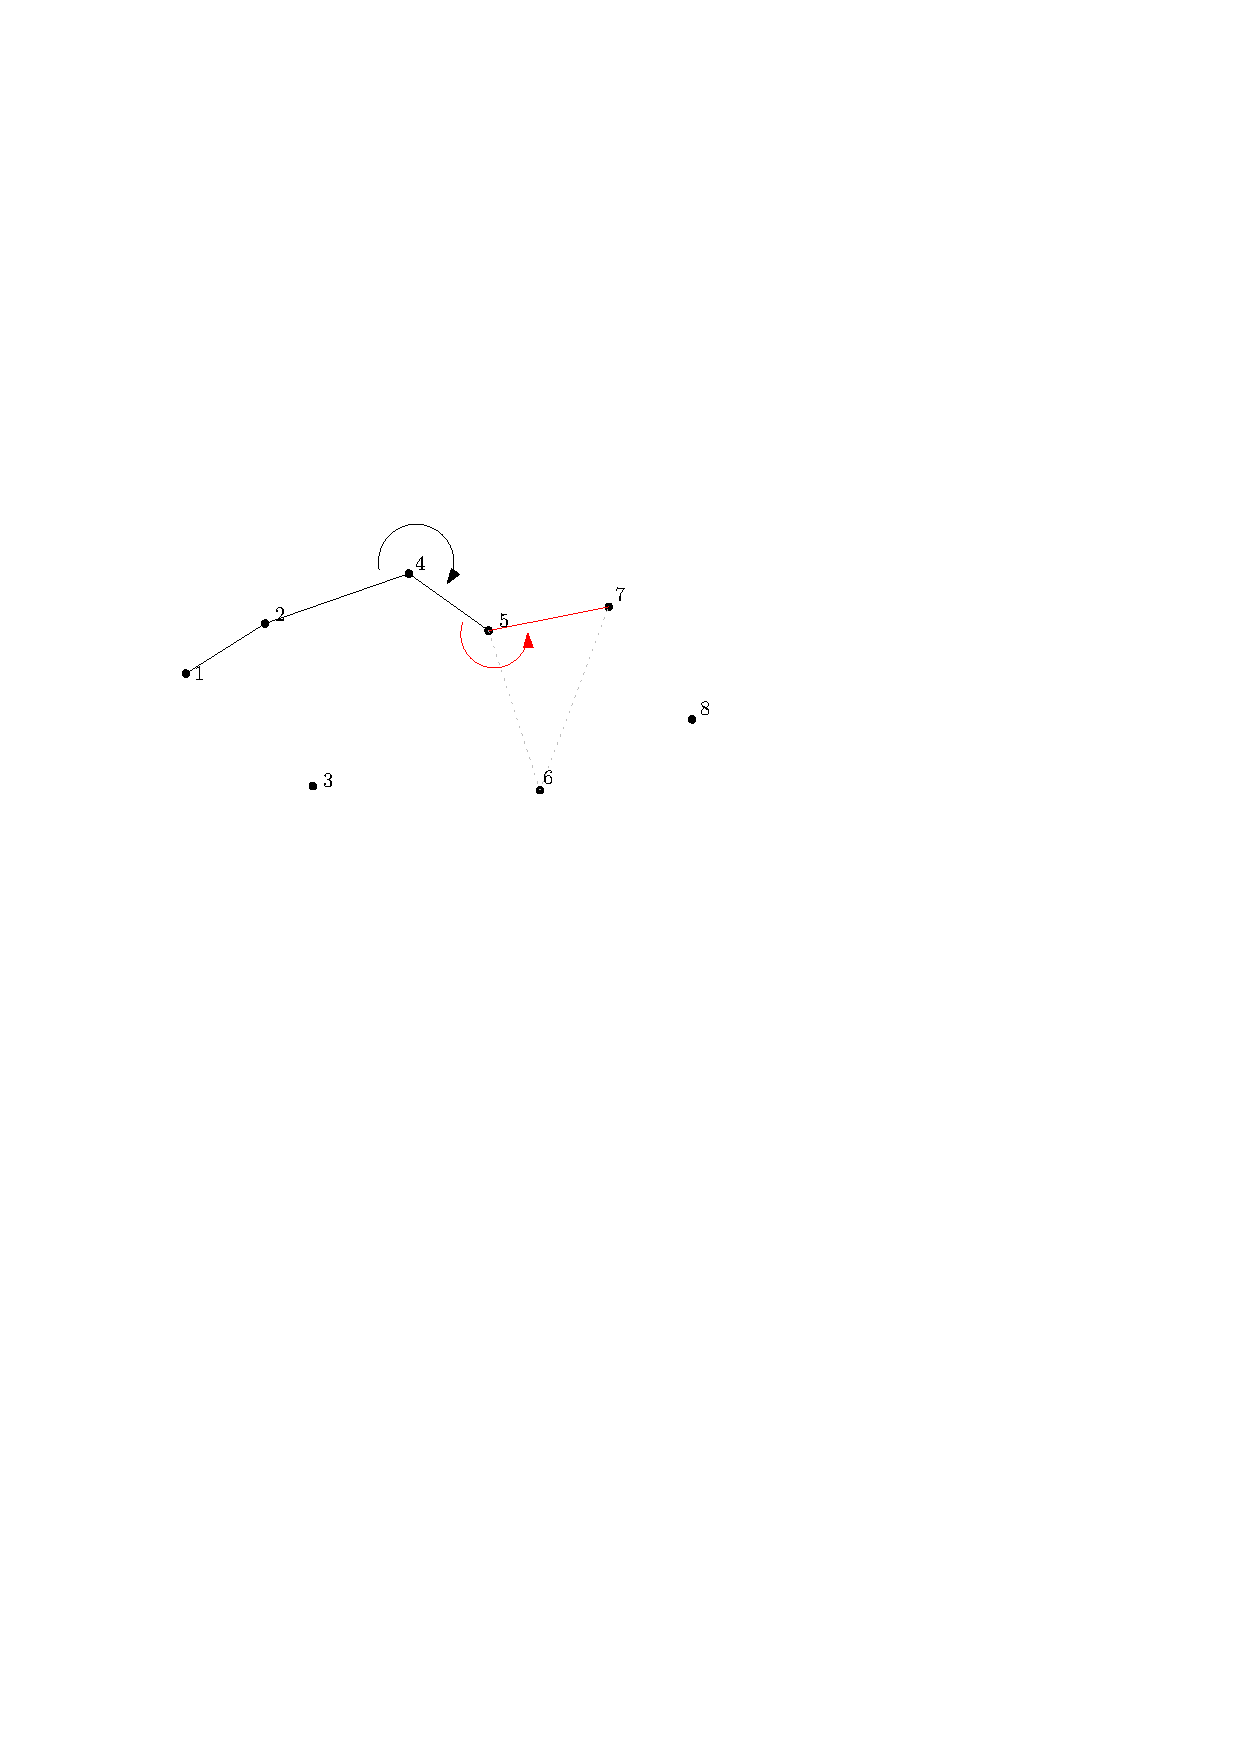
\includegraphics[width=.8\linewidth]{bilder/graham7}
	\end{center}
\end{figure}
\end{frame}


\begin{frame}
	\frametitle{{Graham Scan}}
\begin{figure}[htbp]
	\begin{center}
  	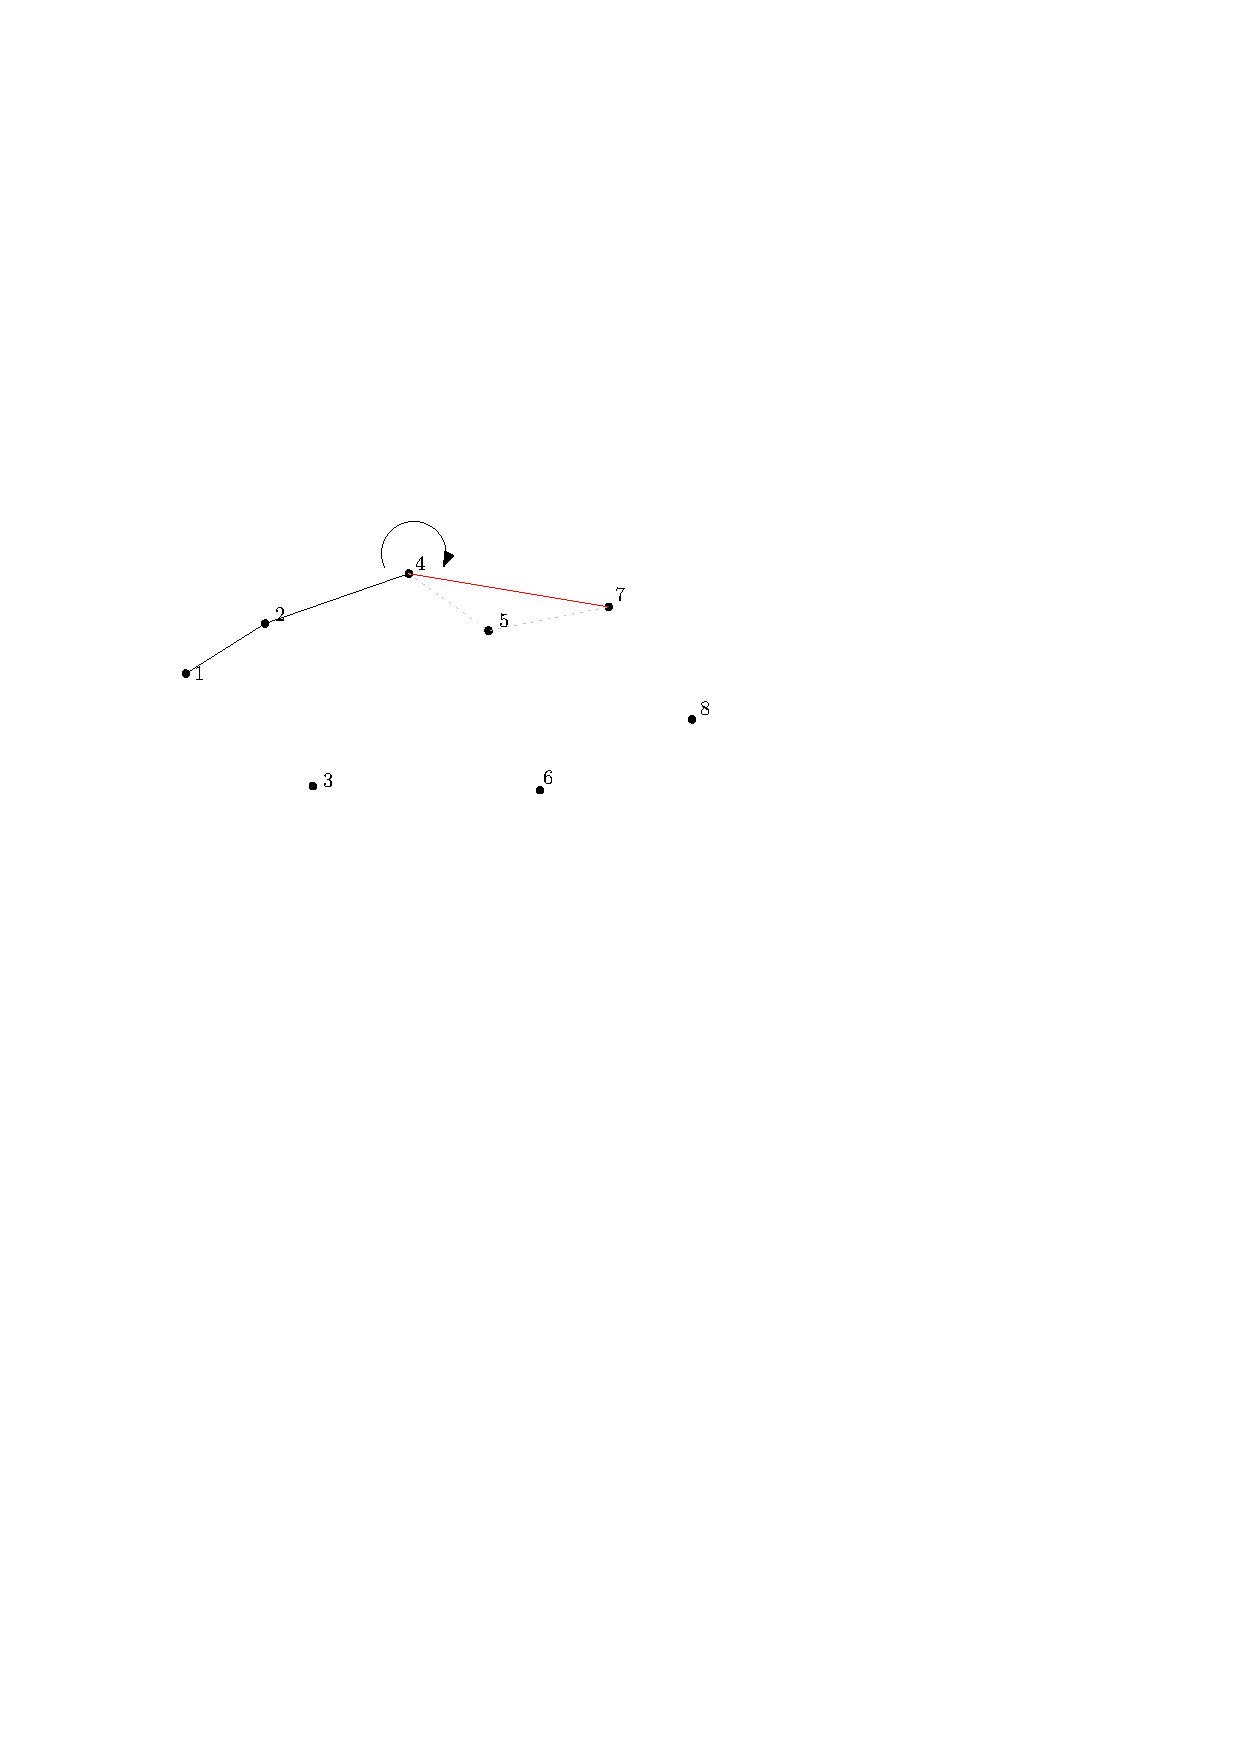
\includegraphics[width=.8\linewidth]{bilder/graham8}
	\end{center}
\end{figure}
\end{frame}

\begin{frame}
	\frametitle{{Graham Scan}}
\begin{figure}[htbp]
	\begin{center}
  	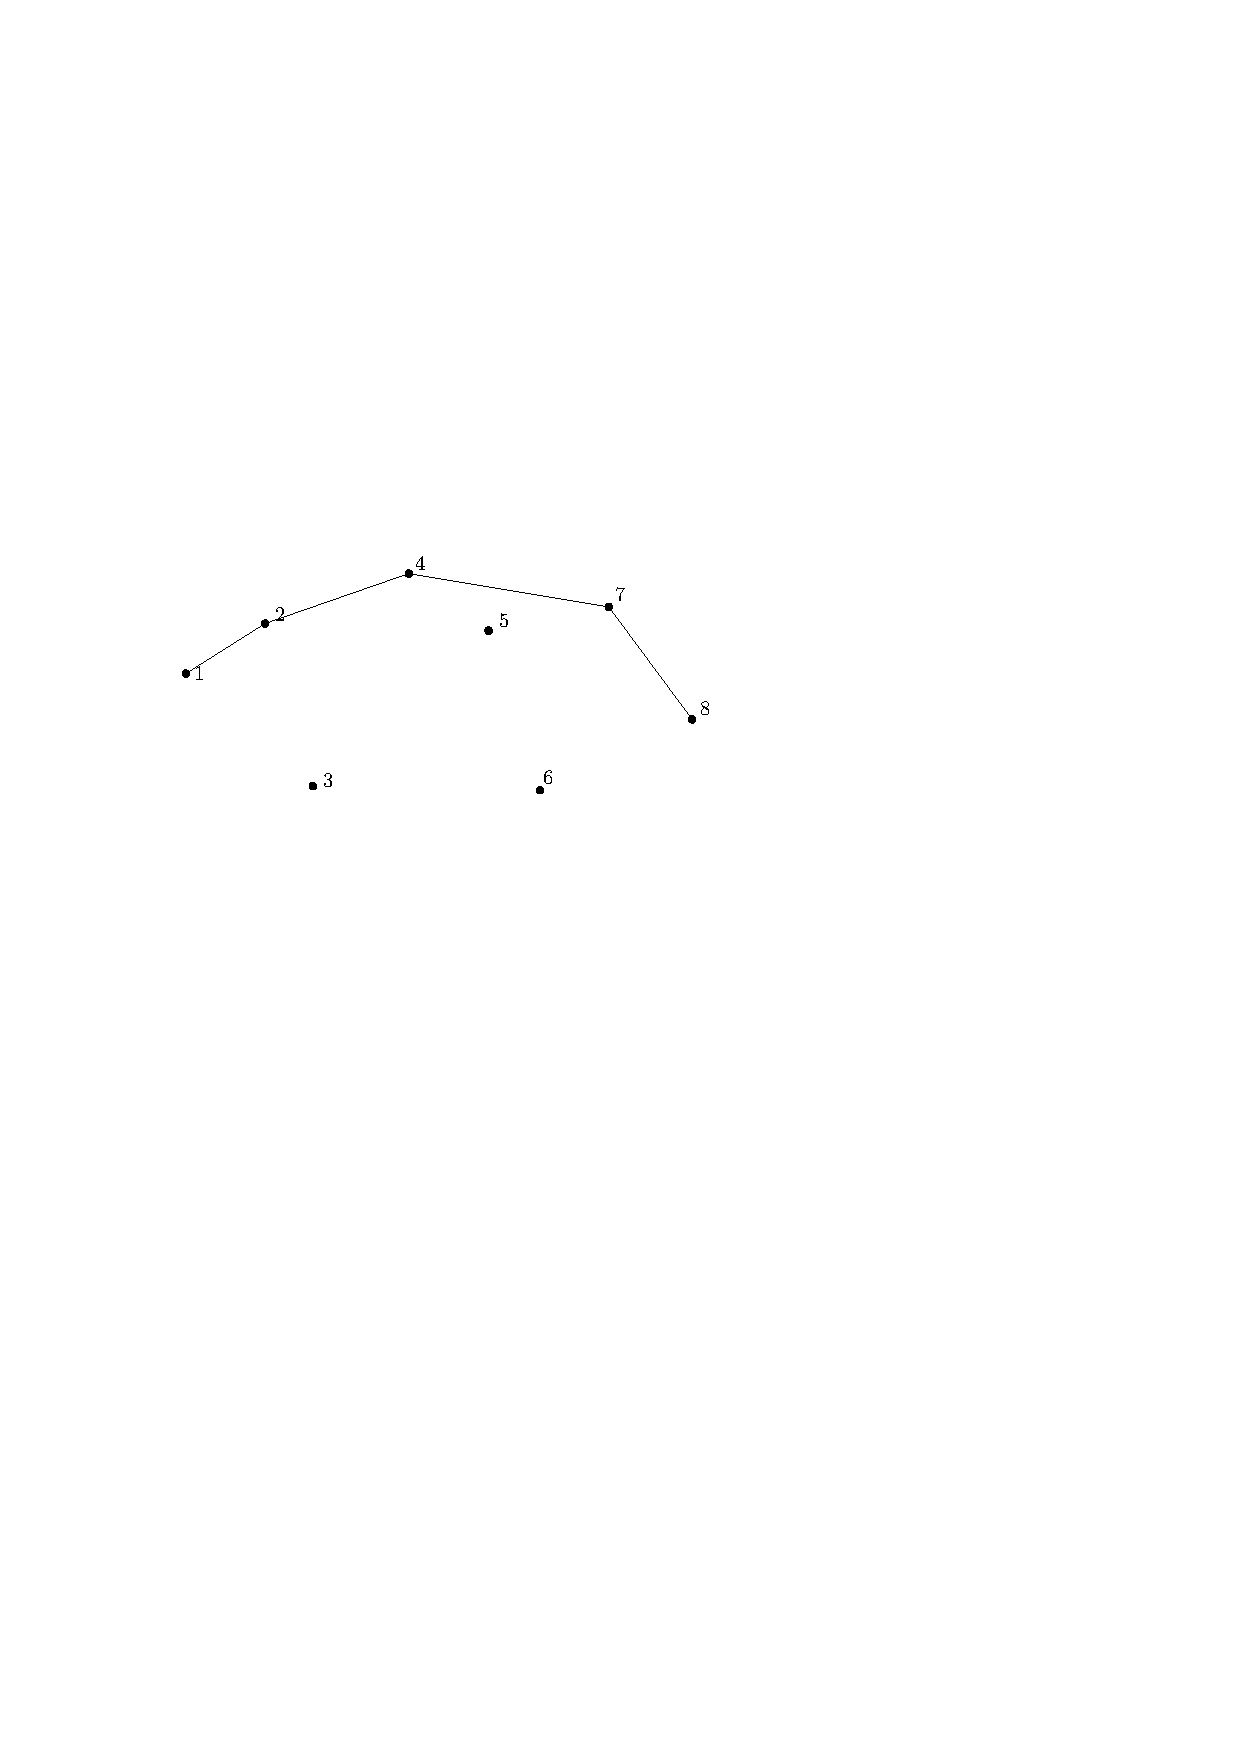
\includegraphics[width=.8\linewidth]{bilder/graham9}
	\end{center}
\end{figure}
\end{frame}

\begin{frame}
	\frametitle{{Noch eine paar letzte Sonderfälle}}
\begin{figure}[htbp]
  \centering
  \begin{minipage}[b]{.4\linewidth}
    
\includegraphics[width=\linewidth]{bilder/sonderfall1}
    \\
    \\
    \tiny{3 Punkte auf einer Geraden $\Rightarrow$ muss wie eine Linksabbiegung interpretiert werden}
  \end{minipage}
  \hfill
  \pause
  \begin{minipage}[b]{.4\linewidth}
    
\includegraphics[width=\linewidth]{bilder/sonderfall2}
    \\
    \\
    \tiny{2 Punkte mit gleichem x-Wert $\Rightarrow$ Punkte müssen lexikographisch sortiert sein}
    \end{minipage}
\end{figure}


\end{frame}


\begin{frame}
	\frametitle{{Graham Scan - Pseudocode}}
TODO: Pseudocode!
\end{frame}



\begin{frame}
	\frametitle{{Graham Scan - Pseudocode}}
TODO: Pseudocode!
\end{frame}

\begin{frame}
	\frametitle{{Graham Scan - Kurze Beweisskizze}}
\textbf{Beweis:}
Man kann zeigen, dass der Algorithmus richtig ist, in dem man zeigt, dass die \textit{UpperHull}, die der Algorithmus findet, richtig ist.\newline \newline
Dies zeigt man mit vollständiger Induktion, in dem man zeigt, dass in der n-ten Iteration die UpperHull der Punkte $p_1$ bis $p_n$ gefunden werden.
\newline
\newline
\pause
\textbf{Laufzeit:}
Die Laufzeit des Graham Scan liegt in $O(n * log (n))$
\end{frame}
